% !TeX root = ./../main.tex

\chapter{Metoda PDU: redukcja błędów wyznaczana eksperymentalnie}\label{chapter:pdu}

\agentinfo{
Rozdział przedstawia główny wkład metodyczny pracy: funkcję odwracania zniekształceń fazy (Phase Distortion Unraveling, PDU).
Źródła:
artykuł ICCS 2022 \agentref{bib:werner_experiment_driven_2022} \agentref{artykuły/Quantum_Errors_ICCS/main.tex},
praca magisterska autora \agentref{artykuły/magisterka_werner_final/chapters/02.tex} \agentref{artykuły/magisterka_werner_final/chapters/03.tex} \agentref{artykuły/magisterka_werner_final/chapters/04.tex},
rysunki \agentref{artykuły/magisterka_werner_final/graf/Eksperymenty} \agentref{artykuły/Quantum_Errors_ICCS/imgs}.
Oryginalnego kodu ani surowych danych nie ma: wszystkie liczby pochodzą z tekstu, tabel i rysunków obu źródeł, a pochodzenie każdej z nich opisuje komentarz w tym pliku (linie zaczynające się od słowa ŹRÓDŁO).
Tekst wykomentowany w źródle artykułu nie jest traktowany jako opublikowany wynik.
Stan: sekcje 4.1--4.5 napisane w zadaniu PHD-TS-40, rysunki i tabele w PHD-TS-42, sekcje 4.6--4.7 w PHD-TS-41, sekcje 4.8--4.9 w PHD-TS-57; poprawki po niezależnej recenzji \agentref{eksperymenty/recenzje/rozdzial-4.md} wprowadzono w zadaniu PHD-TS-91 (2026-11-27), wykaz ustaleń i ich statusów: \agentref{eksperymenty/recenzje/rozdzial-4-poprawki.md}; cały rozdział czeka na przegląd autora.
Skrócenie z 18 do 16 stron: zadanie PHD-TS-97 (2026-11-27), wykaz wyciętych fragmentów, objętość i zapas: \agentref{eksperymenty/recenzje/rozdzial-4-skracanie.md}; każde cięcie da się przywrócić z poprzedniej wersji pliku w repozytorium.
W zadaniu PHD-TS-97 przeniesiono do dodatku trzy rysunki bez zmian treści i podpisów (plik \agentref{chapters/appendix_results_pdu2.tex}, sekcja app:results:pdu2): schemat blokowy fig:pdu:flowchart, wykres fig:pdu:pearson i przykład fig:pdu:two-comp; schemat blokowy wrócił do sekcji 4.5 decyzją autora z 2026-11-28, DO DECYZJI AUTORA, czy dwa pozostałe tam zostają (powrót któregokolwiek do rozdziału wymaga innego cięcia o podobnej wielkości).
Po recenzji (PHD-TS-91): wnioski o stabilności i o przenoszeniu korekty doprowadzono do poziomu danych, rozbieżności źródeł nazwano w tekście i zestawiono w dodatku (tabela tab:pdu:app:discrepancies), a odczyty z rysunków rastrowych są w tekście oznaczone jako odczyty (skrypty recenzenta: \agentref{eksperymenty/recenzje/_robocze/PHD-TS-62}, wyniki powtórzone: \agentref{eksperymenty/recenzje/_robocze/PHD-TS-91}).
Pytania do autora, każde jako zadanie w miejscu, którego dotyczy: podział wkładu w pracy ICCS (4.1); kontrola układu kubitów i transpilacji (4.6, środowisko); definicja próbki w testach korelacji (4.6, miary); odsetek 56 procent dla urządzenia Santiago (4.7.2); do czego odnoszą się liczby przykładu z urządzenia Quito (4.7.3); na jakich obwodach wyznaczano poprawkę dla składnika o częstotliwości 2 i dla szeregu dwuskładnikowego (4.7.4).
Decyzja autora z 2026-11-27: PDU jest metodą rozwijaną w ramach tego doktoratu i ważnym wkładem rozprawy, a jej wyróżnikami względem metod pokrewnych (sekcja 3.3) są korekta indeksowana znanym argumentem, wyznaczana raz dla rodziny obwodów, oraz zbadanie stabilności błędu między kalibracjami urządzenia.
Zakres potwierdzenia pierwszego wyróżnika (ustalenie I1 recenzji): dane rozdziału potwierdzają wyznaczanie korekty raz dla rodziny obwodów tylko dla obwodów jednej funkcji różniących się konfiguracją wejścia; napisano to w sekcjach 4.7.4, 4.8 i 4.9, a wyróżnik pozostaje.
Decyzje redakcyjne DO POTWIERDZENIA PRZEZ AUTORA:
(1) konwencja znaku: błąd to wartość zmierzona minus oczekiwana, a korekta to odjęcie funkcji PDU (artykuł definiuje błąd tak samo, ale mówi o sumie rozkładu i PDU; praca magisterska raz odejmuje, raz dodaje, a jej pseudokod przechowuje różnicę o przeciwnym znaku); niespójność źródeł jest nazwana w sekcji 4.4;
(2) dziedziną funkcji referencyjnej jest przedział od -pi do pi, jak w eksperymentach i w podrozdziale 2.4 (artykuł podaje przedział od -1 do 1 i kąty bramek bez czynnika pi).
Notacja i nazwy są zgodne z podrozdziałem 2.4 \agentref{chapters/theoretical_background_04_QSAMP.tex}: rejestr argumentu o m kubitach, kubit odczytu a, składnik cosinusowy, obwód składnika, znormalizowany histogram.
Definicje wspólne (eksperyment próbkowania, kodowanie argumentu, obwód składnika, twierdzenie o odczycie, rozkład błędu na składową systematyczną i statystyczną) są w rozdziale 2 i tutaj się ich nie powtarza.
Terminologia (uzgodnienie z orkiestratorem): krok metody wykonywany po pomiarze to korekta wyniku, a nie korekcja; słowo korekcja jest zastrzeżone dla QEC (podrozdział 2.3) i pozostaje tylko w dosłownych tytułach sekcji źródeł.
Etykiety do wykorzystania w rozdziałach 5--8: def:pdu:reference-function, def:pdu:errors, def:pdu:function, def:pdu:correction, def:pdu:general; założenia itm:pdu:Z1 do itm:pdu:Z8; wzory eq:pdu:decomposition, eq:pdu:stability, eq:pdu:error, eq:pdu:correction, eq:pdu:residual, eq:pdu:criterion; algorytmy alg:pdu:calibration i alg:pdu:correction; rysunek fig:pdu:flowchart (sekcja 4.5).
Miejsce rozróżnienia argumentu znanego i wartości wyznaczanej, do którego ma się odwoływać rozdział 5: założenie itm:pdu:Z7 oraz akapit par:pdu:known-argument w sekcji 4.4; założenie przenoszalności błędu: itm:pdu:Z8.
}

\section{Cel i zakres rozdziału}\label{sec:pdu:scope}
\agentinfo{
Pytania badawcze rozdziału: PB1 (stabilność błędu między kalibracjami) i PB2 (przenoszalność korekty na inne obliczenia na tym samym układzie kubitów).
Tezy rozprawy są robocze, dlatego tekst odwołuje się do pytań badawczych i do podrozdziału z tezami, bez przytaczania brzmienia tezy T1.
Po ustaleniu ostatecznych tez uzgodnić brzmienie PB1 i PB2 oraz zdanie o tezie z wprowadzeniem \agentref{chapters/introduction.tex}.
}

Rozdział przedstawia funkcję odwracania zniekształceń fazy (ang. \english{Phase Distortion Unraveling}, PDU): metodę redukcji błędów w obliczeniach opartych na próbkowaniu kwantowym, w której poprawkę wyniku wyznacza się eksperymentalnie, a stosuje po stronie klasycznej, już po pomiarze.
Metodę opublikowano w pracy trzech autorów~\cite{werner_experiment_driven_2022}, której pierwszym autorem jest autor rozprawy, a szerzej opisano w jego pracy magisterskiej~\cite{werner_magisterka_2022}.
Rozdział porządkuje jej definicje, jawnie wypisuje założenia, podaje procedurę wraz z kosztem i uzupełnia opis wyników o analizę statystyczną.
PDU jest metodą \glslink{error-reduction}{redukcji błędów} w sensie definicji~\ref{def:tb03:reduction}: nie koduje informacji w kubitach logicznych i nie zmienia wykonywanego obwodu.
\agenttask{
Pytanie do autora (recenzja rozdziału 4, ustalenie I10): jaki był podział wkładu między trzech autorów pracy ICCS 2022 (sformułowanie metody, eksperymenty, analiza wyników)?
Po odpowiedzi dopisać w tym akapicie jedno zdanie o podziale wkładu i uzgodnić je z sekcją 3.3, która mówi o metodzie opracowanej przez autora rozprawy wraz ze współautorami; do tego czasu tekst podaje tylko fakty bibliograficzne.
}

Wynikiem obliczeń opartych na próbkowaniu (podrozdział~\ref{subsec:tb:qsamp:sampling}) nie jest pojedynczy odczyt rejestru, lecz rozkład prawdopodobieństwa estymowany z wielu powtórzeń tego samego obwodu.
Jeżeli składowa systematyczna błędu takiego wyniku zmienia się wolno w porównaniu z odstępem między kolejnymi kalibracjami urządzenia, to można ją zmierzyć raz, na obwodzie o znanym wyniku, i odejmować od wyników późniejszych obliczeń.
Prowadzi to do dwóch pytań badawczych.
\begin{description}
\item[PB1] Czy błąd obliczeń opartych na próbkowaniu kwantowym jest stabilny między kalibracjami urządzenia w stopniu pozwalającym wyznaczyć jego korektę eksperymentalnie?
\item[PB2] Czy korekta wyznaczona dla funkcji referencyjnej poprawia wyniki innych obliczeń wykonywanych na tym samym układzie kubitów?
\end{description}
Odpowiedzi na oba pytania są materiałem dowodowym dla pierwszej z tez rozprawy, dotyczącej redukcji błędów opartej na pomiarze (podrozdział~\ref{sec:introduction:theses}).

Zakres rozdziału obejmuje obwody metody QCoSamp z jednym kubitem odczytu (podrozdział~\ref{subsec:tb:qsamp:qcosamp}), wykonywane w latach 2021--2022 na pięcio- i siedmiokubitowych urządzeniach nadprzewodzących IBM Quantum.
Metoda QCoSamp pochodzi z pracy~\cite{wereszczynski_cosine_2020} i nie jest wkładem autora rozprawy; wkładem jest funkcja PDU, procedura jej kalibracji i stosowania oraz badania eksperymentalne.

\section{Założenia metody}\label{sec:pdu:assumptions}
\agentinfo{
Założenia Z1--Z8 mają etykiety itm:pdu:Z1 do itm:pdu:Z8.
Założenia Z7 (znany argument korekty) i Z8 (przenoszalność błędu) wyodrębniono na polecenie orkiestratora: rozdzielają to, co jest znane w chwili korekty (argument funkcji PDU, kodowany przez wykonującego obliczenie), od tego, co się wyznacza (wartość wyniku), oraz nazywają osobno hipotezę, że błąd funkcji referencyjnej przenosi się na inne obliczenia.
Rozdział nie rozstrzyga kwestii korekty obrazów, w której argumentem funkcji PDU jest wartość piksela oryginału (otwarta sprawa rozdziału 5, opisana w CLAUDE.md).
Rozkład błędu na składową systematyczną, jej dryf i składową statystyczną (wzory eq:pdu:decomposition i eq:pdu:stability) rozszerza o zależność od czasu rozkład z podrozdziału 2.1 (eq:tb01:errordecomp, tam: błąd sprzętowy i błąd statystyczny); jest formalizacją dodaną w rozprawie, bo artykuł i praca magisterska formułują założenie stabilności opisowo.
Po recenzji (ustalenia I3 i I4, PHD-TS-91) rozkład zapisano dla obwodu kalibracyjnego, prawdziwą składową systematyczną oznaczono epsilon z kreską (odróżnioną od funkcji PDU, czyli wielkości zmierzonej i interpolowanej), dryf obejmuje także fluktuacje między seriami, a błąd przenoszenia na inne obliczenia opisano słownie w sekcji 4.4, bez nowego symbolu.
Zdanie o zamianie kubitów zaadaptowano z pracy magisterskiej (rozdz. 2, sekcja PDU) i ze wstępu artykułu; zdanie o prostocie obliczeniowej metody (wstęp artykułu) usunięto przy skracaniu w zadaniu PHD-TS-97.
}

Metoda PDU opiera się na ośmiu założeniach: trzy pierwsze określają klasę obliczeń, trzy kolejne warunki ważności poprawki i koszt metody, a dwa ostatnie sam krok korekty.
\begin{enumerate}
\renewcommand{\theenumi}{Z\arabic{enumi}}
\renewcommand{\labelenumi}{(\theenumi)}
\item\label{itm:pdu:Z1} \emph{Obliczenia oparte na próbkowaniu.}
Wynikiem obliczenia jest znormalizowany histogram stanów bazowych uzyskany z $\nshots$ powtórzeń obwodu (definicja~\ref{def:tb:qsamp:sampling}), interpretowany jako wartość funkcji.
PDU koryguje estymaty prawdopodobieństw, a nie wyniki pojedynczych powtórzeń.
\item\label{itm:pdu:Z2} \emph{Obwód jako czarna skrzynka.}
Obwód jest traktowany jako całość realizująca rozwiązanie określonego problemu.
Metoda nie korzysta z modelu szumu poszczególnych bramek ani z tomografii bramek lub detektora, jest więc zorientowana na problem, a nie na bramkę (kryterium K6 w podrozdziale~\ref{subsec:tb:qec:cost}).
Funkcję PDU wyznacza się dla konkretnej rodziny obwodów, urządzenia i układu kubitów.
\item\label{itm:pdu:Z3} \emph{Znane wartości oczekiwane.}
Istnieje zbiór argumentów, dla których wartości oczekiwane wyniku są znane, na przykład wyznaczone klasycznie; na tym zbiorze przeprowadza się kalibrację.
\item\label{itm:pdu:Z4} \emph{Stabilność błędu.}
Składowa systematyczna błędu wyniku nie zmienia się istotnie między kolejnymi kalibracjami fizycznymi urządzenia (podrozdział~\ref{subsec:tb:noise:sources}).
\item\label{itm:pdu:Z5} \emph{Ten sam układ kubitów.}
Obliczenie korygowane jest wykonywane na tych samych kubitach fizycznych i przy tym samym przypisaniu ról kubitom co obwody kalibracyjne.
\item\label{itm:pdu:Z6} \emph{Brak dodatkowych zasobów kwantowych.}
Obwód obliczeniowy nie zawiera dodatkowych kubitów ani bramek służących korekcji błędów, więc wszystkie kubity i cała dopuszczalna głębokość obwodu pozostają dostępne dla obliczeń.
Kosztem metody są wyłącznie dodatkowe wykonania obwodów kalibracyjnych i obliczenia klasyczne.
\item\label{itm:pdu:Z7} \emph{Znany argument korekty.}
W chwili korekty znany jest argument, dla którego odczytuje się funkcję PDU: konfiguracja wejścia i wynikająca z niej faza kubitu odczytu, które wykonujący obliczenie sam koduje w obwodzie.
Korekta nie korzysta z wartości, którą obliczenie ma wyznaczyć; wartości oczekiwane są potrzebne tylko w kalibracji, zgodnie z założeniem~(\ref{itm:pdu:Z3}), i przy ocenie błędu.
\item\label{itm:pdu:Z8} \emph{Przenoszalność błędu.}
Błąd wyznaczony dla funkcji referencyjnej opisuje także błąd innych obliczeń wykonywanych na tym samym układzie kubitów, przy tej samej fazie kubitu odczytu.
\end{enumerate}

Założenie~(\ref{itm:pdu:Z4}) można zapisać ilościowo, uzupełniając rozkład błędu wyniku na błąd statystyczny i systematyczny błąd sprzętowy (równanie~\eqref{eq:tb01:errordecomp}) o zależność od czasu.
Niech $\tilde{f}_t(x)$ oznacza wynik obwodu kalibracyjnego funkcji $f$ (założenie~\ref{itm:pdu:Z3}) uzyskany dla argumentu $x$ w chwili $t$, a $t_0$ chwilę kalibracji funkcji PDU.
Wtedy
\begin{equation}\label{eq:pdu:decomposition}
\tilde{f}_t(x)=f(x)+\bar{\pdu}(x)+\delta_t(x)+\xi_t(x),
\end{equation}
gdzie $\bar{\pdu}(x)$ jest składową systematyczną błędu w chwili $t_0$, $\delta_t(x)$ jej dryfem, czyli zmianą od tej chwili, powolną albo fluktuującą między kolejnymi seriami ($\delta_{t_0}\equiv 0$), a $\xi_t(x)$ składową statystyczną o zerowej wartości oczekiwanej.
Założenie~(\ref{itm:pdu:Z4}) oznacza, że w okresie między kalibracjami fizycznymi średni kwadrat dryfu jest mały w porównaniu ze średnim kwadratem składowej systematycznej:
\begin{equation}\label{eq:pdu:stability}
\bigl\langle\delta_t^2\bigr\rangle\ll\bigl\langle\bar{\pdu}^{\,2}\bigr\rangle,
\end{equation}
gdzie $\langle\cdot\rangle$ oznacza średnią po argumentach.
Czy warunek~\eqref{eq:pdu:stability} jest spełniony, rozstrzyga się eksperymentalnie (pytanie PB1, podrozdział~\ref{subsec:pdu:results:stability}).
Drugą hipotezą empiryczną jest założenie~(\ref{itm:pdu:Z8}), którego dotyczy pytanie PB2 (podrozdziały~\ref{subsec:pdu:results:one} i~\ref{subsec:pdu:results:two}).

Z założeń wynikają granice metody.
PDU usuwa wyłącznie powtarzalną część błędu: nie odtwarza informacji utraconej wskutek dekoherencji, nie zmniejsza rozrzutu wyników i nie stosuje się do algorytmów, w których liczy się wynik pojedynczego wykonania obwodu.
Wymaga ponownej kalibracji po każdej zmianie naruszającej założenie~(\ref{itm:pdu:Z4}) lub~(\ref{itm:pdu:Z5}), czyli po kalibracji fizycznej urządzenia, po zmianie układu kubitów i po zmianie sposobu transpilacji obwodu (podrozdział~\ref{subsec:tb:gates}).
Funkcja PDU zawiera bowiem łącznie błędy poszczególnych kubitów i błędy wynikające z zależności między nimi, toteż już zamiana miejscami dwóch kubitów może wymagać wyznaczenia jej od nowa~\cite{werner_experiment_driven_2022,werner_magisterka_2022}.
Krok metody wykonywany po pomiarze nazywa się w rozprawie korektą wyniku (podrozdział~\ref{subsec:tb:qec:taxonomy}).

\section{Funkcja referencyjna i wyznaczanie błędu}\label{sec:pdu:reference}
\agentinfo{
Funkcja referencyjna to składnik cosinusowy o n=1 i r=0, a obwód referencyjny to obwód tego składnika; obie definicje ogólne są w podrozdziale 2.4, więc tutaj jest tylko odwołanie.
Definicję funkcji wyznaczonej i zbioru błędów wyznaczonych odtworzono z definicji wykomentowanych w źródle artykułu (sekcja Materials and methods) i z opisu w pracy magisterskiej (rozdz. 2, sekcja PDU), w notacji rozprawy.
Liczba powtórzeń 8192 pochodzi wyłącznie z przypisu w artykule; praca magisterska liczby powtórzeń nie podaje (DO POTWIERDZENIA PRZEZ AUTORA, czy wszystkie eksperymenty wykonano z 8192 powtórzeniami).
Wartości 0,0055 oraz 3,1e-5 są obliczeniem dodanym w rozprawie ze wzoru na wariancję estymatora częstości (eq:tb01:estimator).
Schemat obwodu referencyjnego: zgodnie z uzgodnieniem z orkiestratorem rozdział odwołuje się do rysunku obwodu składnika z podrozdziału 2.4 (fig:tb:qsamp:component), żeby nie dublować rysunków; wariant z zaznaczonymi etapami powstawania błędu dla węzła D=0010 jest przygotowany w pliku \agentref{rozprawa/figures/chp_pdu/pdu_reference_circuit.tex}, ale nie jest włączony do tekstu (DO DECYZJI AUTORA).
}

Kalibracja wymaga obwodu o wyniku znanym dla całej siatki argumentów (założenie~\ref{itm:pdu:Z3}); w metodzie PDU jest nim najprostszy obwód metody QCoSamp, czyli obwód jednego składnika cosinusowego (definicje~\ref{def:tb:qsamp:component} i~\ref{def:tb:qsamp:circuit}).

\begin{Definition}[Funkcja referencyjna i obwód referencyjny]\label{def:pdu:reference-function}
\glslink{reference-function}{Funkcją referencyjną} nazywamy funkcję $\reffun$ odwzorowującą przedział $[-\pi,\pi)$ w przedział $[0,1]$, realizowaną przez obwód kwantowy w modelu próbkowania, której wartości w $K$ węzłach $x_0<\dots<x_{K-1}$ są znane niezależnie od tego obwodu.
Obwód ten nazywamy obwodem referencyjnym.
W niniejszej pracy funkcją referencyjną jest składnik cosinusowy o częstotliwości $n=1$ i fazie $r=0$,
\begin{equation}\label{eq:pdu:reffun}
\reffun(x)=\coscomp_{1,0}(x)=\frac{1+\cos x}{2},
\end{equation}
a obwodem referencyjnym obwód składnika $\compcirc_{1,0}(D)$.
\end{Definition}

Węzłami są argumenty $x_D$ kodowane ciągami bitów $D$ w rejestrze argumentu o $m$ kubitach (definicja~\ref{def:tb:qsamp:argument}), czyli $K=2^{m}$ punktów siatki $X_m=\{x_D\colon D\in\{0,1\}^m\}$ o kroku $\pi/2^{m-1}$.
Dla urządzeń pięciokubitowych użytych w eksperymentach $m=4$ (obwód referencyjny przedstawia rysunek~\ref{fig:tb:qsamp:component}), co daje $16$ węzłów od $-\pi$ do $\tfrac{7}{8}\pi$ z krokiem $\tfrac{1}{8}\pi$.
% ŹRÓDŁO: artykuły/magisterka_werner_final/chapters/03.tex, sekcja ,,Korekcja funkcji jednej zmiennej'' (zakres x i skok) oraz listing lst:python_cos_phi (kąty bramek).
Z twierdzenia~\ref{thm:tb:qsamp:readout} wynika, że na urządzeniu idealnym prawdopodobieństwo wyniku $0$ na kubicie odczytu jest równe $\reffun(x_D)$.
Argument jest zapisany w fazie lokalnej kubitu odczytu i zamieniany na prawdopodobieństwo przez interferencję (podrozdział~\ref{subsec:tb:phase}); stąd w nazwie metody mowa o zniekształceniach fazy.

\begin{Definition}[Funkcja wyznaczona i zbiór błędów wyznaczonych]\label{def:pdu:errors}
Niech $\tilde{\prob}_D$ oznacza znormalizowany histogram eksperymentu próbkowania o liczbie powtórzeń $\nshots$, wykonanego dla obwodu referencyjnego $\compcirc_{1,0}(D)$.
Funkcją wyznaczoną nazywamy funkcję $\reffunexp\colon X_m\to[0,1]$ daną wzorem $\reffunexp(x_D)=\tilde{\prob}_D(\ket{0}_a)$.
Błędem wyznaczonym w węźle $x_D$ nazywamy liczbę
\begin{equation}\label{eq:pdu:error}
\pdu_D=\reffunexp(x_D)-\reffun(x_D),
\end{equation}
a zbiorem błędów wyznaczonych zbiór par $\mathcal{V}_m=\{(x_D,\pdu_D)\colon D\in\{0,1\}^m\}$.
\end{Definition}

Błąd wyznaczony jest sumą składowej systematycznej, która jest przedmiotem korekty, i składowej statystycznej estymatora $\tilde{\prob}_D$, czyli $\pdu_D=\bar{\pdu}(x_D)+\xi_{t_0}(x_D)$; odchylenie standardowe drugiej z nich nie przekracza $1/(2\sqrt{\nshots})$ (równanie~\eqref{eq:tb01:estimator}).
Według pracy~\cite{werner_experiment_driven_2022} w eksperymentach przyjęto $\nshots=8192$.
% ŹRÓDŁO: artykuły/Quantum_Errors_ICCS/main.tex, przypis w sekcji ,,Materials and methods'' (8.192 repetitions, maximal number on IBM Q Experience); w artykuły/magisterka_werner_final/chapters/02.tex--05.tex liczba powtórzeń nie występuje (sprawdzono wyszukiwaniem, PHD-TS-91).
Odchylenie to nie przekracza wtedy $0{,}0055$, a wkład składowej statystycznej do błędu średniokwadratowego wartości $1/(4\nshots)\approx 3{,}1\cdot 10^{-5}$.
% ŹRÓDŁO: obliczenie własne: 1/(2*sqrt(8192)) = 0,00552; 1/(4*8192) = 3,05e-5.
Błędy średniokwadratowe obserwowane na urządzeniach są rzędu $10^{-2}$ (podrozdział~\ref{subsec:pdu:results:stability}), czyli o ponad dwa rzędy wielkości większe: o dokładności kalibracji decyduje sprzęt, a nie próbkowanie.

\section{Definicja funkcji PDU}\label{sec:pdu:definition}
\agentinfo{
Przyjęta konwencja znaku (błąd = zmierzone minus oczekiwane, korekta = odjęcie) wymaga potwierdzenia autora; opis rozbieżności w konspekcie rozdziału.
Definicja def:pdu:general przenosi do notacji rozprawy ogólną definicję z pracy CoDIT 2025 \agentref{artykuły/CoDIT_2025_final_paper/root.tex} (sekcja Error reduction); warunek minimalności całki z tamtej definicji zastąpiono jawnym operatorem interpolacji, bo w oryginalnym zapisie nie wyznacza on funkcji jednoznacznie (DO DECYZJI AUTORA).
Skróty z zadań PHD-TS-91 i PHD-TS-97 (wykazy w plikach wskazanych w konspekcie rozdziału): szczegóły niespójności znaku w źródłach są w tabeli w dodatku; porównanie interpolacji liniowej i sześciennej ściśnięto do jednego zdania.
Dodane w rozprawie, nieobecne w źródłach (do akceptacji autora): wzór na błąd wyniku skorygowanego eq:pdu:residual, warunek opłacalności eq:pdu:criterion, postać funkcji PDU w modelu z kontrastem i przesunięciem fazy (model pochodzi z podrozdziału 2.2, eq:tb:noise:fringe), własność zerowania się sumy błędów po stanach bazy, porównanie interpolacji liniowej i sześciennej.
W eksperymentach z lat 2021--2022 funkcję PDU stosowano jako tablicę błędów w węzłach (praca magisterska, rozdz. 2); interpolację sześcienną wprowadza dopiero praca CoDIT 2025.
Źródła różnie opisują, czy wynik dla cos(2x) korygowano tablicą wyznaczoną na cos(x) i indeksowaną fazą (tak opisuje to artykuł), czy tablicą wyznaczoną na tych samych obwodach cos(2x) (tak opisują to tekst i pseudokod pracy magisterskiej); tekst definicji obejmuje oba warianty.
Odczyt rysunku fig:pdu:example (recenzja, ustalenie I1; powtórzony w PHD-TS-91) jest zgodny z drugim wariantem i niezgodny z pierwszym; tekst sekcji 4.7.4 podaje to jako odczyt jednego przykładu, a pytanie do autora jest w zadaniu w tamtej sekcji.
}

Funkcja PDU rozszerza zbiór błędów wyznaczonych z węzłów siatki na całą dziedzinę.

\begin{Definition}[Funkcja PDU kubitu]\label{def:pdu:function}
Niech $\mathcal{V}_m$ będzie zbiorem błędów wyznaczonych dla obwodu referencyjnego na ustalonym urządzeniu i ustalonym układzie kubitów, a $\mathcal{I}$ ustalonym operatorem interpolacji funkcji okresowych o okresie $2\pi$.
\glslink{pdu-function}{Funkcją odwracania zniekształceń fazy} (funkcją PDU) kubitu odczytu nazywamy funkcję
\begin{equation}\label{eq:pdu:function}
\pdu=\mathcal{I}[\mathcal{V}_m]\colon\mathbb{R}\to\mathbb{R},
\qquad
\pdu(x_D)=\pdu_D\quad\text{dla każdego } D\in\{0,1\}^m .
\end{equation}
\end{Definition}

\begin{Definition}[Wynik skorygowany]\label{def:pdu:correction}
Niech $\tilde{f}$ będzie wynikiem obliczenia w modelu próbkowania, wykonanego na urządzeniu i układzie kubitów, dla których wyznaczono funkcję $\pdu$, a $\varphi$ fazą lokalną kubitu odczytu, którą to obliczenie zamienia na prawdopodobieństwo.
Wynikiem skorygowanym nazywamy liczbę
\begin{equation}\label{eq:pdu:correction}
\hat{f}=\tilde{f}-\pdu(\varphi).
\end{equation}
W szczególności dla funkcji referencyjnej $\reffuncorr(x)=\reffunexp(x)-\pdu(x)$.
\end{Definition}

\paragraph{Co musi być znane w chwili korekty.}\label{par:pdu:known-argument}
Wzór~\eqref{eq:pdu:correction} rozdziela dwie wielkości: argument $\varphi$, dla którego odczytuje się funkcję PDU, i wartość $\hat{f}$, którą się wyznacza.
Argument musi być znany niezależnie od wyniku pomiaru (założenie~\ref{itm:pdu:Z7}).
Dla składnika $\coscomp_{n,r}$ jest nim $nx+r$ sprowadzone do przedziału $[-\pi,\pi)$, czyli suma kątów bramek przesunięcia fazy działających na kubit odczytu w konfiguracji wejścia zakodowanej przez wykonującego obliczenie~\cite{werner_magisterka_2022}; odjęcie $\pdu(\varphi)$ nie wymaga więc znajomości wartości wyznaczanej.
To, że błąd wyznaczony na funkcji referencyjnej jest właściwą poprawką dla innego obliczenia o tej samej fazie, jest osobnym założeniem~(\ref{itm:pdu:Z8}).
Jeżeli faza kubitu odczytu zależy od danych nieznanych temu, kto koryguje wynik, definicji~\ref{def:pdu:correction} nie można zastosować wprost; przypadek ten wykracza poza eksperymenty tego rozdziału.

Źródła nie są w sprawie znaku poprawki jednolite ani wewnętrznie spójne (dodatek, tabela~\ref{tab:pdu:app:discrepancies}); rozprawa stosuje konsekwentnie definicje~\ref{def:pdu:errors} i~\ref{def:pdu:correction}.
% ŹRÓDŁO: ICCS main.tex, streszczenie (the final result after correction is the sum of PDF and PDU) i sekcja Materials and methods (epsilon(x) = gamma-tilde(x) - gamma(x)); magisterka 02.tex, sekcja PDU (znalezioną wartość należy odjąć) oraz 03.tex, sekcja ,,Korekcja funkcji jednej zmiennej'' (dodawano wartość; listing lst:experiment_1: oczekiwany_wynik - wynik, wynik + blad).
Wynik skorygowany może nieznacznie wyjść poza przedział $[0,1]$, gdy wartość oczekiwana leży blisko jego krańca (rysunek~\ref{fig:pdu:example}); jeżeli ma być dalej interpretowany jako prawdopodobieństwo, należy go zrzutować na ten przedział.

Dla obwodu kalibracyjnego z rozkładu~\eqref{eq:pdu:decomposition} i wzoru~\eqref{eq:pdu:correction} wynika błąd wyniku skorygowanego w chwili $t$:
\begin{equation}\label{eq:pdu:residual}
\hat{f}_t(x)-f(x)=\delta_t(x)+\iota(x)+\xi_t(x)-\xi_{t_0}(x),
\end{equation}
gdzie $\iota(x)$ jest błędem interpolacji, równym zeru w węzłach, a $\xi_{t_0}$ składową statystyczną kalibracji.
Korekta zastępuje więc składową systematyczną błędu jej dryfem, za cenę podwojenia wariancji składowej statystycznej.
Uśredniając kwadraty po argumentach, otrzymujemy warunek wystarczający na to, by korekta zmniejszała błąd średniokwadratowy wyniku obwodu kalibracyjnego:
\begin{equation}\label{eq:pdu:criterion}
\bigl\langle(\bar{\pdu}+\delta_t)^2\bigr\rangle-\bigl\langle(\delta_t+\iota)^2\bigr\rangle>\frac{1}{4\nshots}.
\end{equation}
Przy $\nshots=8192$ prawa strona wynosi około $3{,}1\cdot10^{-5}$, więc o opłacalności korekty decyduje w praktyce relacja między składową systematyczną błędu a jej dryfem, czyli założenie~(\ref{itm:pdu:Z4}).
Dla obliczeń innych niż kalibracyjne dochodzi do tego błąd przenoszenia, czyli różnica między składową systematyczną ich błędu a funkcją PDU odczytaną dla ich fazy, pomijalna tylko na mocy założenia~(\ref{itm:pdu:Z8}).

\paragraph{Co zawiera funkcja PDU.}
Błąd wyznaczony w węźle $x_D$ jest wypadkową wszystkich zjawisk na drodze od przygotowania stanu do odczytu: błędów bramek, dekoherencji, przesłuchu i błędu odczytu (podrozdział~\ref{subsec:tb:noise:sources}).
Zależność błędu od fazy widać już w modelu~\eqref{eq:tb:noise:fringe}, w którym szum zmniejsza widoczność interferencji do $v$ i przesuwa fazę o $\cohangle$: funkcja PDU ma wtedy postać $\pdu(x)=\tfrac{1}{2}\bigl[v\cos(x+\cohangle)-\cos x\bigr]$ i znika tożsamościowo tylko dla $v=1$ i $\cohangle=0$.
W rzeczywistym obwodzie różne ciągi $D$ uaktywniają różne bramki, więc błąd zależy od konfiguracji wejścia nie tylko poprzez fazę, i właśnie dlatego funkcję PDU wyznacza się z pomiaru, a nie z modelu.

\begin{Definition}[Funkcja PDU układu]\label{def:pdu:general}
Niech $\mathbb{E}$ będzie bazą pomiarową podukładu kubitów, $\tilde{\prob}(\ket{\psi};x_k)$ znormalizowanym histogramem stanu $\ket{\psi}\in\mathbb{E}$ uzyskanym dla fazy $x_k$, a $\prob(\ket{\psi};x_k)$ odpowiadającą mu wartością oczekiwaną.
Funkcją PDU układu nazywamy funkcję $\pdu\colon\mathbb{E}\times\mathbb{R}\to\mathbb{R}$, która dla każdego ustalonego stanu $\ket{\psi}$ jest funkcją PDU w sensie definicji~\ref{def:pdu:function}, wyznaczoną z par
\begin{equation}\label{eq:pdu:general}
\bigl(x_k,\ \tilde{\prob}(\ket{\psi};x_k)-\prob(\ket{\psi};x_k)\bigr),\qquad k=0,\dots,K-1 .
\end{equation}
\end{Definition}

Funkcja PDU kubitu jest przypadkiem szczególnym, w którym $\mathbb{E}=\{\ket{0},\ket{1}\}$ oraz $\pdu(\ket{1},x)=-\pdu(\ket{0},x)$.
W ogólności błędy wyznaczone sumują się w każdym węźle po stanach bazy do zera, bo oba rozkłady są unormowane; jeżeli operator $\mathcal{I}$ jest liniowy względem wartości w węzłach, własność tę ma także funkcja PDU, a rozkład skorygowany pozostaje unormowany, o ile nie zastosowano rzutowania na przedział $[0,1]$.
Postać ogólną sformułowano w pracy~\cite{werner_error_reduction_2025} z myślą o kodowaniu obrazów, z warunkiem minimalności całki w miejscu operatora interpolacji; jej zastosowanie, w tym pytanie o to, jaki argument jest w niej znany w chwili korekty, jest przedmiotem rozdziału~\ref{chapter:pdu_images}.
% ŹRÓDŁO: artykuły/CoDIT_2025_final_paper/root.tex, sekcja ,,Error reduction'', definicja General PDU function (warunek z całką po przedziale od -pi do pi).

\paragraph{Wybór interpolacji i gęstość węzłów.}
W eksperymentach opisanych w tym rozdziale funkcję PDU stosowano wyłącznie w węzłach siatki, jako tablicę błędów wyznaczonych odczytywaną dla konfiguracji wejścia $D$~\cite{werner_magisterka_2022}, bo argumenty wszystkich korygowanych obliczeń należały do siatki.
% ŹRÓDŁO: artykuły/magisterka_werner_final/chapters/02.tex, sekcja PDU (określić, dla jakiej wartości D otrzymano wynik, i znaleźć odpowiadającą mu wartość epsilon_D w zbiorze v).
Gdy faza wypada między węzłami, interpolacja odcinkami liniowa nie wzmacnia błędu statystycznego węzłów i dla gładkiej funkcji błędu ma błąd rzędu $h^{2}$ ($h$: krok siatki), a okresowa funkcja sklejana trzeciego stopnia, przyjęta w pracy~\cite{werner_error_reduction_2025}, zmniejsza go do rzędu $h^{4}$, lecz przenosi zaburzenie pojedynczego węzła na sąsiednie przedziały.
Gęstość węzłów ogranicza rejestr argumentu: $K=2^{m}$, a każdy dodatkowy kubit rejestru podwaja koszt kalibracji i dodaje do obwodu bramkę kontrolowaną.

\section{Procedura kalibracji i korekty}\label{sec:pdu:procedure}
\agentinfo{
Algorytmy alg:pdu:calibration i alg:pdu:correction porządkują procedurę opisaną słownie w pracy magisterskiej (rozdz. 2, sekcja PDU) i jej pseudokod (rozdz. 3, listing lst:experiment_1); schemat blokowy fig:pdu:flowchart narysowano na nowo w TikZ \agentref{rozprawa/figures/chp_pdu/pdu_flowchart.tex}, w zadaniu PHD-TS-97 przeniesiono go do dodatku, a decyzją autora z 2026-11-28 wrócił do tej sekcji.
Koszt kalibracji (16 obwodów, 131072 powtórzenia) to obliczenie z liczb źródłowych: 16 obwodów (praca magisterska) razy 8192 powtórzenia (artykuł).
Limit 100 obwodów w jednym zadaniu pochodzi z pracy magisterskiej (rozdz. 3, sekcja Macierze sąsiedztwa).
Praca magisterska podaje liczbę obwodów pełnej kalibracji dwóch rejestrów jako 2 do potęgi n razy m; poprawna wartość to 2 do potęgi n plus m (64 obwody dla dwóch rejestrów po 3 kubity) i taką podano w tekście.
Propozycja do dyskusji w sekcji 4.8 (usunięta z tekstu z braku miejsca): test kontrolny, czyli ponowny pomiar kilku węzłów i porównanie błędów z zapamiętanymi jako praktyczne sprawdzenie warunku ponownej kalibracji; w eksperymentach nie był stosowany.
Słowa kluczowe pseudokodu przetłumaczono lokalnie w obu algorytmach; jeśli inne rozdziały też używają algpseudocode, warto przenieść tłumaczenia do config/my-settings.tex (zgłoszone w raporcie).
Po recenzji (ustalenia I7, I8, D1 i D7; PHD-TS-91): akapit o warunku ponownej kalibracji formułuje regułę warunkowo (w eksperymentach przyjmowano) i odróżnia kalibrację ustalającą nowe wartości błędów (według źródeł raz na dobę, w pracy magisterskiej ze słowem prawdopodobnie) od częstszych kalibracji deklarowanych przez dostawcę; warunek w algorytmie alg:pdu:correction obejmuje zmianę transpilacji; na schemacie fig:pdu:flowchart sprawdzenie warunku poprzedza korektę, jak w algorytmie; zdanie o kalibracji rejestrów z osobna nie przesądza już przyczyny niepowodzenia eksperymentu E5.
Źródła nie mówią wprost, którego z dwóch zdarzeń dotyczy reguła; przyjęto kalibrację ustalającą błędy, bo tak opisują ją wyniki obu źródeł (DO POTWIERDZENIA PRZEZ AUTORA).
}

Stosowanie metody składa się z dwóch faz: kalibracji, wykonywanej raz po każdej kalibracji fizycznej urządzenia (algorytm~\ref{alg:pdu:calibration}), oraz korekty, wykonywanej dla każdego wyniku obliczeń (algorytm~\ref{alg:pdu:correction}); ich powiązanie w cyklu pracy urządzenia przedstawia rysunek~\ref{fig:pdu:flowchart}.

\begin{algorithm}[tb]
\algrenewcommand\algorithmicrequire{\textbf{Wejście:}}
\algrenewcommand\algorithmicensure{\textbf{Wyjście:}}
\algrenewcommand\algorithmicfor{\textbf{dla}}
\algrenewcommand\algorithmicdo{\textbf{wykonaj}}
\algrenewcommand\algorithmicend{\textbf{koniec}}
\algrenewcommand\algorithmicreturn{\textbf{zwróć}}
\caption{Kalibracja funkcji PDU}\label{alg:pdu:calibration}
\begin{algorithmic}[1]
\Require urządzenie $B$, układ kubitów $L$, liczba kubitów rejestru argumentu $m$, liczba powtórzeń $\nshots$, funkcja referencyjna $\reffun$, operator interpolacji $\mathcal{I}$
\Ensure funkcja PDU $\pdu$ dla pary $(B,L)$, chwila kalibracji $t_0$
\State $\mathcal{V}_m\gets\emptyset$
\For{każdego $D\in\{0,1\}^m$}
  \State zbuduj obwód referencyjny $\compcirc_{1,0}(D)$ i przypisz go do kubitów $L$ urządzenia $B$
\EndFor
\State wykonaj wszystkie $2^{m}$ obwodów na urządzeniu $B$, każdy $\nshots$ razy, i zapisz chwilę $t_0$
\For{każdego $D\in\{0,1\}^m$}
  \State $\reffunexp(x_D)\gets\tilde{\prob}_D(\ket{0}_a)$ \Comment{znormalizowany histogram}
  \State $\pdu_D\gets\reffunexp(x_D)-\reffun(x_D)$ \Comment{błąd wyznaczony}
  \State $\mathcal{V}_m\gets\mathcal{V}_m\cup\{(x_D,\pdu_D)\}$
\EndFor
\State $\pdu\gets\mathcal{I}[\mathcal{V}_m]$
\State \Return $\pdu$, $t_0$
\end{algorithmic}
\end{algorithm}

\begin{algorithm}[tb]
\algrenewcommand\algorithmicrequire{\textbf{Wejście:}}
\algrenewcommand\algorithmicensure{\textbf{Wyjście:}}
\algrenewcommand\algorithmicif{\textbf{jeżeli}}
\algrenewcommand\algorithmicthen{\textbf{to}}
\algrenewcommand\algorithmicend{\textbf{koniec}}
\algrenewcommand\algorithmicreturn{\textbf{zwróć}}
\caption{Korekta wyniku obliczenia funkcją PDU}\label{alg:pdu:correction}
\begin{algorithmic}[1]
\Require funkcja PDU $\pdu$ z chwilą kalibracji $t_0$ dla pary $(B,L)$; wynik $\tilde{f}$ obliczenia wykonanego na $(B,L)$ w chwili $t$; faza $\varphi$ kubitu odczytu, znana z konstrukcji obwodu (założenie~\ref{itm:pdu:Z7})
\Ensure wynik skorygowany $\hat{f}$ albo żądanie ponownej kalibracji
\If{między $t_0$ a $t$ nastąpiła kalibracja fizyczna urządzenia $B$ albo zmienił się układ kubitów $L$ lub sposób transpilacji}
  \State \Return żądanie ponownej kalibracji (algorytm~\ref{alg:pdu:calibration})
\EndIf
\State sprowadź $\varphi$ do przedziału $[-\pi,\pi)$
\State $\hat{f}\gets\tilde{f}-\pdu(\varphi)$
\State opcjonalnie: $\hat{f}\gets\min\{1,\max\{0,\hat{f}\}\}$ \Comment{rzutowanie na $[0,1]$}
\State \Return $\hat{f}$
\end{algorithmic}
\end{algorithm}

\begin{figure}[tb]
\centering
% !TeX root = ./../../main.tex
% Schemat blokowy procedury kalibracji i korekty metodą PDU (rysunek fig:pdu:flowchart).
% Rysunek własny, narysowany na nowo w TikZ na potrzeby rozprawy.
% Treść odpowiada algorytmom alg:pdu:calibration i alg:pdu:correction z chapters/pdu.tex.
% Wymaga bibliotek TikZ: arrows.meta, calc, positioning (wczytane w config/my-settings.tex).
\begin{tikzpicture}[
  node distance=5mm and 10mm,
  nohyph/.style={execute at begin node={\hyphenpenalty=10000\relax\exhyphenpenalty=10000\relax}},
  box/.style={draw, rounded corners=2pt, align=center, font=\footnotesize, nohyph, minimum height=10mm, text width=52mm, inner sep=3pt},
  qbox/.style={box, fill=black!10},
  cbox/.style={box, fill=white},
  arr/.style={-{Stealth[length=2mm]}, semithick},
  lab/.style={font=\footnotesize\itshape, inner sep=1.5pt},
]
% --- faza kalibracji (lewa kolumna) ---
\node[qbox] (phys) {Kalibracja fizyczna urządzenia\\(wykonuje dostawca)};
\node[qbox, below=of phys] (run) {Wykonanie $2^{m}$ obwodów referencyjnych\\$\compcirc_{1,0}(D)$, każdy $\nshots$ razy};
\node[cbox, below=of run] (err) {Wyznaczenie błędów\\$\pdu_D=\reffunexp(x_D)-\reffun(x_D)$};
\node[cbox, below=of err] (int) {Interpolacja: funkcja PDU\\$\pdu=\mathcal{I}[\mathcal{V}_m]$, zapis chwili $t_0$};
% --- faza korekty (prawa kolumna) ---
% Kolejność jak w algorytmie alg:pdu:correction: najpierw sprawdzenie warunku ponownej kalibracji, potem korekta.
\node[qbox, right=18mm of phys] (comp) {Wykonanie obwodu obliczeniowego:\\wynik $\tilde{f}$, znana faza $\varphi$};
\coordinate (dc) at ($(comp.south)+(0,-18.5mm)$);
\draw[fill=white] ($(dc)+(-29mm,0)$) coordinate (dW) -- ($(dc)+(0,14.5mm)$) coordinate (dN) -- ($(dc)+(29mm,0)$) coordinate (dE) -- ($(dc)+(0,-14.5mm)$) coordinate (dS) -- cycle;
\node[align=center, font=\footnotesize, inner sep=0pt] at (dc) {Nowa kalibracja\\fizyczna, zmiana\\układu kubitów\\lub transpilacji?};
\node[cbox, anchor=north] (corr) at ($(dS)+(0,-4mm)$) {Korekta po stronie klasycznej:\\$\hat{f}=\tilde{f}-\pdu(\varphi)$};
\coordinate (low) at ($(corr.south)+(0,-3.5mm)$);
\coordinate (rw) at ($(run.west)+(-6mm,0)$);
% --- przepływ ---
\draw[arr] (phys) -- (run);
\draw[arr] (run) -- (err);
\draw[arr] (err) -- (int);
\draw[arr] (int.east) -- ++(9mm,0) |- (comp.west);
\draw[arr] (comp.south) -- (dN);
\draw[arr] (dS) -- (corr.north);
\node[lab, anchor=north west] at ($(dS)+(0.5mm,0)$) {nie};
\draw[arr] (corr.east) -- ++(4mm,0) |- (comp.east);
\draw[arr] (dW) -- ++(-4mm,0) coordinate (t1) -- (t1 |- low) -- (rw |- low) -- (rw) -- (run.west);
\node[lab, anchor=south east] at ($(dW)+(0,0.5mm)$) {tak};
% --- nazwy faz ---
\node[lab, anchor=south] at ($(phys.north)+(0,1.5mm)$) {faza kalibracji};
\node[lab, anchor=south] at ($(comp.north)+(0,1.5mm)$) {faza korekty};
% --- legenda ---
\node[qbox, text width=6mm, minimum height=4mm, anchor=north west] (lq) at ($(phys.south west)+(0,-57mm)$) {};
\node[font=\footnotesize, anchor=west] at (lq.east) {urządzenie kwantowe};
\node[cbox, text width=6mm, minimum height=4mm, anchor=west] (lc) at ($(lq.east)+(36mm,0)$) {};
\node[font=\footnotesize, anchor=west] at (lc.east) {komputer klasyczny};
\end{tikzpicture}

\caption[Schemat blokowy kalibracji i korekty metodą PDU]{Schemat blokowy kalibracji i korekty metodą PDU.
Bloki szare są wykonywane na urządzeniu kwantowym, bloki białe na komputerze klasycznym.
Opracowanie własne.}
\label{fig:pdu:flowchart}
\end{figure}

\paragraph{Koszt.}
Spośród kryteriów zasobów kwantowych K1--K3 z podrozdziału~\ref{subsec:tb:qec:cost} metoda obciąża tylko K3, czyli dodatkowe wykonania obwodu, i to wyłącznie w fazie kalibracji (założenie~\ref{itm:pdu:Z6}).
Kalibracja wymaga wykonania $K=2^{m}$ obwodów referencyjnych, czyli $K\nshots$ powtórzeń: dla $m=4$ i $\nshots=8192$ jest to $16$ obwodów i $131\,072$ powtórzenia, co mieści się w jednym zadaniu przesyłanym do urządzenia.
% ŹRÓDŁO: 16 obwodów: magisterka 03.tex; 8192: przypis w ICCS main.tex; limit 100 obwodów na zadanie: magisterka 03.tex, sekcja ,,Macierze sąsiedztwa''; iloczyn 131072 to obliczenie własne.
Narzut nie zależy od głębokości obwodu obliczeniowego, rośnie natomiast wykładniczo z rozmiarem rejestru argumentu.
Dla dwóch rejestrów argumentów, liczących $m$ i $m'$ kubitów, pełna kalibracja wymaga $2^{m+m'}$ obwodów, a kalibracja każdego rejestru z osobna tylko $2^{m}+2^{m'}$; drugi wariant nie poprawił jednak wyników (podrozdział~\ref{subsec:pdu:results:two}).

\paragraph{Warunek ponownej kalibracji.}
W eksperymentach przyjmowano, że funkcja PDU zachowuje ważność do najbliższej kalibracji ustalającej nowe wartości błędów urządzenia~\cite{werner_experiment_driven_2022,werner_magisterka_2022}.
Źródła odróżniają ją od częstszych kalibracji deklarowanych przez dostawcę (na rysunku~\ref{fig:pdu:app:scatter} w dodatku czas od takiej kalibracji nie przekracza trzech godzin): deklarowane błędy bramek zmieniały się raz na dobę, a w ciągu dnia urządzenia były prawdopodobnie tylko dostrajane.
% ŹRÓDŁO: ICCS main.tex, sekcja Results (despite information provided by IBM regarding last calibration time, declared error values on gates changed once per day; tests for hours since initial calibration, which set error values on gates); magisterka 03.tex, sekcja ,,Stabilizacja błędów w czasie'' (korelacja błędu z czasem od pierwszej kalibracji danego dnia; kalibracja raz dziennie i mniejsze kalibracje w ciągu dnia, w źródle ze słowem ,,prawdopodobnie''); trzy godziny: odczyt z osi rysunków pdu_scatter_manila.png (punkty do około 66 minut) i pdu_scatter_santiago.png (do około 175 minut).
Przy tym rozumieniu reguła oznacza jedną kalibrację PDU na dobę dla każdej pary urządzenia i układu kubitów, a algorytm~\ref{alg:pdu:correction} sprawdza ją na podstawie informacji podawanych przez dostawcę; zastrzeżenia omawia podrozdział~\ref{sec:pdu:discussion}.

\section{Metodyka badań eksperymentalnych}\label{sec:pdu:methodology}
\agentinfo{
Źródła: praca magisterska \agentref{artykuły/magisterka_werner_final/chapters/02.tex} (Środowisko eksperymentalne, Metodologia) \agentref{artykuły/magisterka_werner_final/chapters/03.tex} (protokoły) oraz artykuł \agentref{artykuły/Quantum_Errors_ICCS/main.tex} (Experimental protocol).
Daty wycofania urządzeń potwierdzono 2026-11-26 w dokumentacji IBM Quantum \agentref{bib:ibm_retired_qpus_2026}; parametrów urządzeń nie podano, bo nie ma ich w źródłach.
Od zadania PHD-TS-97 akapit Środowisko nie wylicza urządzeń, dat ich wycofania ani wersji biblioteki Qiskit (0.36.2 jako najnowsza w czasie pisania pracy magisterskiej): odsyła do tabel tab:app:env:devices i tab:app:env:software oraz tekstu dodatku A \agentref{chapters/appendix_experiments.tex}, w którym te dane są ze źródłami.
Rozbieżności źródeł zgłoszone w komentarzu do PHD-TS-41 (DO DECYZJI AUTORA):
okres zbierania danych w eksperymencie stabilności (praca magisterska: luty 2021 -- maj 2022; artykuł: 05.2021 -- 01.2022);
lista urządzeń (artykuł raz wymienia sześć urządzeń bez Athens, raz siedem; praca magisterska dodaje cztery urządzenia siedmiokubitowe);
liczba serii po kalibracji w eksperymencie korekty (tekst pracy magisterskiej: 15, jej pseudokod: 10, wykomentowany tekst artykułu: 10);
zakres argumentów w eksperymencie dwóch zmiennych (praca magisterska: do 7/8 pi przy kroku pi/4, co jest niespójne z rejestrem trzech kubitów; przyjęto 8 węzłów na rejestr, od -pi do 3/4 pi);
postać funkcji dwóch zmiennych: praca magisterska podaje (1/2)(1+cos(x+y)), ale komentarze jej pseudokodu wskazują jedno przesunięcie fazy o -pi na kubicie odczytu, co przy kodowaniu obu argumentów od -pi daje fazę x+y+pi, czyli (1/2)(1-cos(x+y)); w tekście przyjęto zapis z pracy magisterskiej, bo tylko on jest w źródle podany wprost, a analiza PDU zależy od fazy kubitu odczytu, a nie od sposobu jej opisu (DO POTWIERDZENIA PRZEZ AUTORA, dla jakiej fazy liczono wartości oczekiwane);
tomografia: 243 obwody odpowiadają pięciu kubitom, a prezentowane macierze są jednokubitowe;
część rysunków w pracy magisterskiej ma daty z czerwca 2022 r. w nazwach plików, czyli po zadeklarowanym końcu zbierania danych (kwiecień i maj 2022 r.).
Przedziały ufności Fishera i uwaga o niewrażliwości korelacji na zniekształcenie afiniczne są dodane w rozprawie.
Po recenzji (ustalenia I6, I11, D4 i D6; PHD-TS-91): tekst mówi, że źródła nie definiują próbki (przyjęta definicja jest rekonstrukcją; liczności 100, 1470, 1667, 1162 i 679 nie są wielokrotnościami 16, co opisano w dodatku), że p-wartości ze źródeł dotyczą hipotezy o braku korelacji, a nie poprawy, i że wnioski sprawdzono także dla liczby serii (N/16 w E3, N/64 w E5; szczegóły w dodatku); dodano zdanie, że źródła nie dokumentują kontroli układu kubitów i transpilacji (założenie Z5); wersję Qiskit podano jako najnowszą w czasie pisania pracy magisterskiej, bo wersji użytej źródło nie podaje.
Niewprowadzone z recenzji (ustalenie I6 d): wariant współczynnika Kendalla przy wiązaniach nie jest w źródłach podany, a wartości oczekiwane mają tylko 9 (cos x) albo 5 (cos 2x) różnych wartości; w tekście jest tylko ogólne zastrzeżenie o rozkładzie w dodatku.
Miary MSE, odchylenie standardowe błędu i współczynnik Pearsona są zdefiniowane w podrozdziale 2.5; współczynniki Kendalla i Spearmana nie mają definicji w rozdziale 2 (do rozważenia: dodać tam jedno zdanie).
}

Badania miały odpowiedzieć na pytania PB1 i PB2 na rzeczywistych urządzeniach i objęły pięć eksperymentów zestawionych w tabeli~\ref{tab:pdu:protocols}.
Ich opis łączy informacje z pracy~\cite{werner_experiment_driven_2022} i z pracy magisterskiej autora~\cite{werner_magisterka_2022}, która opisuje większy zbiór danych; rozbieżności między źródłami zestawia tabela~\ref{tab:pdu:app:discrepancies} w dodatku.
We wszystkich eksperymentach argumenty, a zatem i wartości oczekiwane, były znane dla każdego obwodu, bo tylko wtedy można wyznaczyć błąd: eksperymenty dotyczą założeń~(\ref{itm:pdu:Z4}) i~(\ref{itm:pdu:Z8}), a nie użycia metody do wyznaczenia nieznanej wartości.

\begin{table}[tb]
\centering
\caption[Eksperymenty z metodą PDU]{Eksperymenty z metodą PDU.
Oznaczenia obwodów jak w podrozdziale~\ref{subsec:tb:qsamp:qcosamp}.
Opracowanie własne na podstawie~\cite{werner_experiment_driven_2022,werner_magisterka_2022}.}
\label{tab:pdu:protocols}
\footnotesize
\begin{tabular}{@{}p{0.45cm}>{\raggedright\arraybackslash}p{3.3cm}>{\raggedright\arraybackslash}p{4.5cm}>{\raggedright\arraybackslash}p{3.3cm}p{2.3cm}@{}}
\toprule
 & \textbf{Cel} & \textbf{Obwody} & \textbf{Urządzenia} & \textbf{Okres} \\
\midrule
E1 & stan kubitu odczytu & obwód referencyjny, jeden węzeł; tomografia stanu: $3^{5}=243$ obwody & Quito, Lima, Santiago, Belem & nie podano \\
E2 & stabilność błędu w~czasie (PB1) & obwód referencyjny, 16 węzłów; 15 serii na dobę & pięciokubitowe oraz Lagos, Perth, Casablanca & 02.2021--05.2022 \\
E3 & korekta funkcji jednej zmiennej (PB1, PB2) & $\coscomp_{1,0}$ i $\coscomp_{2,0}$, 16 węzłów; kalibracja i 15 serii & siedem pięciokubitowych & 05.2021--04.2022 \\
E4 & korekta szeregu dwuskładnikowego (PB2) & $\tfrac{1}{2}(\coscomp_{1,0}+\coscomp_{2,0})$, 8 węzłów & Lima & nie podano \\
E5 & korekta funkcji dwóch zmiennych (PB2) & funkcja dwóch zmiennych, 64 obwody; kalibracja na $8+8$ obwodach & Lagos, Casablanca, Perth, Jakarta & nie podano \\
\bottomrule
\end{tabular}
\end{table}
% ŹRÓDŁO tabeli: artykuły/magisterka_werner_final/chapters/03.tex (sekcje: Macierze sąsiedztwa; Stabilizacja błędów w czasie; Korekcja funkcji jednej zmiennej; Korekcja funkcji dwóch zmiennych). Artykuł ICCS podaje dla E2 okres 05.2021--01.2022.

\paragraph{Środowisko.}
Obwody budowano i uruchamiano za pomocą biblioteki Qiskit~\cite{Qiskit} na pięcio- i siedmiokubitowych urządzeniach nadprzewodzących IBM Quantum; urządzenia, okresy badań i oprogramowanie zestawiają tabele~\ref{tab:app:env:devices} i~\ref{tab:app:env:software} w dodatku~\ref{appendix:experiments}.
Wszystkie te urządzenia już wycofano~\cite{ibm_retired_qpus_2026}, więc eksperymentów nie da się powtórzyć na tym samym sprzęcie, a parametrów kalibracyjnych z okresu badań w zachowanych materiałach nie ma.
% ŹRÓDŁO: dokumentacja IBM Quantum, strona ,,Retired cloud QPUs'', odczyt 2026-11-26 (daty wycofania poszczególnych urządzeń: dodatek A, tabela tab:app:env:devices i komentarz źródłowy do jej kolumny ,,Wycofanie'').
Dostęp do urządzeń odbywał się przez wspólną kolejkę zadań, więc chwili wykonania obwodu nie można było zaplanować: odstępy między kolejnymi seriami wynosiły od kilku minut do ponad godziny, a każdy wynik zapisywano razem z czasem od kalibracji deklarowanym przez dostawcę~\cite{werner_magisterka_2022}.
% ŹRÓDŁO: magisterka 03.tex, sekcje ,,Stabilizacja błędów w czasie'' i ,,Korekcja funkcji jednej zmiennej''.
Źródła nie podają, czy między kalibracją funkcji PDU a seriami korygowanymi ustalano przypisanie kubitów i transpilację, więc spełnienia założenia~(\ref{itm:pdu:Z5}) nie da się potwierdzić.
% ŹRÓDŁO: w artykuły/magisterka_werner_final/chapters/02.tex--05.tex i w ICCS main.tex nie ma wzmianki o układzie kubitów ani o ustawieniach transpilacji (sprawdzono wyszukiwaniem, PHD-TS-91).
\agenttask{
Pytanie do autora (recenzja rozdziału 4, ustalenie I11): czy między kalibracją funkcji PDU a seriami korygowanymi przypisanie kubitów fizycznych i ustawienia transpilacji były ustalone na stałe (na przykład jawny układ początkowy i ten sam poziom optymalizacji)?
Po odpowiedzi zastąpić zdanie powyżej opisem tego, jak kontrolowano założenie Z5, i poprawić odpowiednie zdanie w sekcji 4.8.
}

\paragraph{Protokoły.}
W eksperymencie E1 stan kubitu odczytu po wykonaniu obwodu referencyjnego odtwarzano metodą tomografii stanu (podrozdział~\ref{subsec:tb:noise:characterisation}) z użyciem modułu Qiskit Ignis.
% ŹRÓDŁO: magisterka 03.tex, sekcja ,,Macierze sąsiedztwa'' (state_tomography_circuits, StateTomographyFitter, metoda lstsq, 243 układy w trzech zadaniach, limit 100 obwodów na zadanie).
W eksperymencie E2 zestaw obwodów referencyjnych wykonywano w różnym czasie od deklarowanej kalibracji, a zależność błędu średniokwadratowego serii od czasu opisano linią trendu.
W eksperymentach E3 i E4 po kalibracji funkcji PDU zestaw obwodów badanej funkcji wykonywano wielokrotnie i każdy wynik korygowano tablicą błędów wyznaczonych.
Na jakich obwodach wyznaczano tę tablicę dla składnika $\coscomp_{2,0}$, źródła opisują różnie, a dla szeregu, którego obwód ma dwie fazy, więc tablicę można w nim indeksować tylko konfiguracją wejścia, nie podają (podrozdział~\ref{subsec:pdu:results:two}).
% ŹRÓDŁO: ICCS main.tex, akapit Experimental protocol (once experimentally designated correction function basing on one component will improve the results of subsequent components); magisterka 03.tex, sekcja ,,Korekcja funkcji jednej zmiennej'' (15 razy wykonywano zestawy obwodów wykorzystanych podczas uzyskiwania funkcji PDU) i listing lst:experiment_1; dwie fazy: rozprawa, podrozdział 2.4, równanie eq:tb:qsamp:mixture i opis obwodu fig:tb:qsamp:two-components.
W eksperymencie E5 funkcję dwóch zmiennych realizowano z dwoma rejestrami argumentu po trzy kubity, których fazy sumują się na kubicie odczytu (równanie~\eqref{eq:tb:qsamp:two-variables}); w pracy~\cite{werner_magisterka_2022} zapisano ją jako $\tfrac{1}{2}(1+\cos(x+y))$.
% UWAGA: stałe przesunięcie fazy w tym obwodzie nie jest w źródle jednoznaczne (zob. konspekt sekcji); przyjęto zapis z pracy magisterskiej.
Funkcję PDU wyznaczano dla każdego rejestru z osobna, na ośmiu obwodach z bramkami działającymi tylko na ten rejestr, a wynik każdego z 64~obwodów korygowano sumą błędów odpowiadających obu rejestrom.

\paragraph{Miary i analiza statystyczna.}
Jakość wyniku jednej serii opisują błąd średniokwadratowy MSE i odchylenie standardowe błędu $\sigma_e$ (równanie~\eqref{eq:tb:qimg:errors}), liczone po węzłach siatki.
Zgodność wyników z wartościami oczekiwanymi w całym zbiorze danych mierzono współczynnikami korelacji: Pearsona $r$ oraz rangowymi $\tau$ Kendalla i $r_{\mathrm{S}}$ Spearmana~\cite{bib:statistics_wilc}, osobno przed korektą i po korekcie.
Źródła nie definiują próbki; przyjęto, że jest nią para złożona z wyniku dla jednego węzła w jednej serii i jego wartości oczekiwanej.
P-wartości podane w źródłach dotyczą hipotezy o braku korelacji, a nie poprawy po korekcie; poprawę ocenia się w rozprawie $95$-procentowymi przedziałami ufności współczynnika $r$, wyznaczonymi przekształceniem Fishera.
Przedziały te zakładają niezależność próbek, są więc optymistyczne, dlatego wnioski sprawdzono także dla liczby serii w miejsce liczby próbek (dodatek, strona~\pageref{tab:pdu:app:pvalues}).
Współczynnik $r$ jest ponadto niewrażliwy na afiniczne zniekształcenie wyniku, takie jak samo zmniejszenie widoczności interferencji w modelu~\eqref{eq:tb:noise:fringe}: miarą zgodności wartości jest MSE, a korelacja ocenia zgodność kształtu.
% ŹRÓDŁO: liczności z tabeli tab:pdu:corr: 100, 1470, 1667, 1162 i 679 nie dzielą się przez 16 (1248 i 3760 się dzielą), a wszystkie liczności eksperymentu E5 dzielą się przez 64; obliczenie własne.
\agenttask{
Pytanie do autora (recenzja rozdziału 4, ustalenie I6): co było próbką w testach korelacji eksperymentu E3, skoro liczności 100, 1470, 1667, 1162 i 679 nie są wielokrotnościami 16 (niepełne serie czy inna definicja próbki)?
Po odpowiedzi poprawić zdanie o definicji próbki i, jeśli trzeba, sposób szacowania liczby serii.
}

\section{Wyniki}\label{sec:pdu:results}

\subsection{Charakterystyka błędu urządzeń}\label{subsec:pdu:results:devices}
\agentinfo{
Tytuł sekcji źródłowej w pracy magisterskiej to Macierze sąsiedztwa, ale jej treścią są macierze gęstości z tomografii stanu; macierzy sąsiedztwa w źródłach nie ma.
Rysunek fig:pdu:app:density (umieszczony w dodatku z braku miejsca w rozdziale) przeniesiono z pracy magisterskiej \agentref{artykuły/magisterka_werner_final/graf/Eksperymenty/densitymatrix_111_re_graph.png}; ten sam plik jest w katalogu artykułu.
ROZBIEŻNOŚĆ (DO DECYZJI AUTORA): praca magisterska opisuje ten rysunek jako wynik z urządzenia Quito dla argumentu pi, a wykomentowany podpis w źródle artykułu jako wynik z urządzenia Lima dla 7/8 pi; wykomentowana tabela artykułu podaje dla Limy elementy 0.276 i 0.724, zgodne z rysunkiem.
Dlatego tekst i podpis nie wskazują urządzenia ani węzła.
Praca magisterska interpretuje ujemną część urojoną elementu pozadiagonalnego jako niepoprawność macierzy; jest to własność każdej macierzy hermitowskiej, więc tej uwagi nie przeniesiono.
Po recenzji (ustalenie D3, PHD-TS-91): wniosek kontrolny oparto na długości wektora Blocha (około 0,5, obliczona z elementów odczytanych z rysunku), a nie na samej niezerowości elementów pozadiagonalnych; przy węźle 7/8 pi część urojona elementów pozadiagonalnych występuje także w stanie idealnym, więc nie wnioskuje się z niej o błędzie koherentnym.
Dalsze macierze gęstości z pracy magisterskiej mają w podpisie argumenty spoza siatki (5/4 pi, -2 pi) i nie zostały przeniesione.
}

W eksperymencie E1 macierz gęstości kubitu odczytu, odtworzona dla węzła, w którym obwód idealny pozostawia ten kubit w stanie $\ket{1}$ lub bardzo blisko niego, opisuje stan mieszany: elementy diagonalne wynoszą około $0{,}27$ i $0{,}72$, a długość wektora Blocha, obliczona z elementów odczytanych z rysunku, około $0{,}5$ wobec $1$ dla stanu czystego (rysunek~\ref{fig:pdu:app:density} w dodatku).
% ŹRÓDŁO: odczyt z rysunku densitymatrix_111_re_graph.png: elementy diagonalne około 0,27 i 0,72, elementy pozadiagonalne o części rzeczywistej około 0,05 i urojonej około 0,12 co do modułu; długość wektora Blocha: sqrt((0,27-0,72)^2 + (2*0,05)^2 + (2*0,12)^2) = 0,52 (obliczenie własne, PHD-TS-91); wartości 0.276, 0.724, 0.054 i 0.125 podaje wykomentowana tabela w artykuły/Quantum_Errors_ICCS/main.tex (IBMQ Lima), użyta tylko jako potwierdzenie odczytu.
Odstępstwo elementu $\rho_{00}$ od wartości idealnej jest tym samym błędem, który w modelu próbkowania obserwuje się jako błąd wyznaczony $\pdu_D$; macierze uzyskane na pozostałych urządzeniach miały ten sam charakter~\cite{werner_magisterka_2022}.
Wynik ma znaczenie kontrolne: stan kubitu odczytu nie jest maksymalnie mieszany, więc błąd wyniku nie jest skutkiem całkowitej utraty informacji kwantowej.

\subsection{Stabilność błędu w czasie}\label{subsec:pdu:results:stability}
\agentinfo{
Rysunki fig:pdu:trends (a) i (b) przeniesiono bez zmian: (a) z artykułu \agentref{artykuły/Quantum_Errors_ICCS/imgs/time stability.jpg}, (b) z pracy magisterskiej \agentref{artykuły/magisterka_werner_final/graf/Eksperymenty/trendlines2.png}; danych liczbowych linii trendu nie ma, więc nie odtwarzano ich w pgfplots.
Poziomy MSE (0,01--0,06 oraz 0,03--0,12) są odczytane z osi tych rysunków, a nie z danych.
ROZBIEŻNOŚCI (DO DECYZJI AUTORA):
(1) artykuł: ponad 56 procent wartości błędu na urządzeniu Santiago przekraczało średnią o więcej niż 20 procent; praca magisterska: warunek odchylenia do 20 procent spełnia 56 procent wartości; po recenzji (ustalenie B1, PHD-TS-91) tekst podaje obie wersje i odczyt z rysunku rozrzutu w dodatku (Santiago 40--43 procent w paśmie, Manila 82--83 procent), bez wyboru wersji; pytanie do autora jest w zadaniu pod akapitem;
(2) oś czasu: w artykule czas od kalibracji (0--20 h), w pracy magisterskiej godzina doby;
(3) kierunki trendów: artykuł podaje 4 malejące, 2 stałe, 1 rosnący (Quito malejący); praca magisterska: malejące Bogota i Manila, rosnące Perth, Quito, Lima, Casablanca;
(4) poziom MSE dla urządzenia Bogota: około 0,04--0,05 na rysunku z artykułu i około 0,11 na rysunku z pracy magisterskiej;
(5) na rysunku z artykułu zmiana MSE wzdłuż linii trendu dla urządzeń Manila i Belem wynosi 0,021--0,022 (odczyt skryptem recenzenta), czyli nieznacznie więcej niż deklarowany próg 0,02; po recenzji (ustalenie I5) tekst podaje próg jako stwierdzenie artykułu i obok odczyt z rysunku.
Dolne oszacowanie dryfu z nierówności trójkąta i uwaga o nachyleniach są dodane w rozprawie; po recenzji wniosek o braku trendu zastąpiono stwierdzeniem, że bez rozrzutu punktów i niepewności nachyleń nie da się stwierdzić ani trendu, ani jego braku, a wyjaśnienie nachyleń nierównomiernym rozkładem pomiarów podano jako możliwość.
Hipotezy o związku rozrzutu na urządzeniu Santiago z częstszymi kalibracjami nie wpisano (zadanie w sekcji 3.5, które przywołuje wartości 56 i 83 procent; po rozstrzygnięciu pytania o 56 procent trzeba je uzgodnić).
}

Rozrzut pojedynczych pomiarów błędu zależał od urządzenia: na urządzeniu Manila $83\%$ zmierzonych wartości różniło się od średniej o nie więcej niż $20\%$~\cite{werner_experiment_driven_2022,werner_magisterka_2022}, a dla urządzenia Santiago źródła podają tę samą liczbę w przeciwnym znaczeniu: ponad $56\%$ wartości poza takim pasmem~\cite{werner_experiment_driven_2022} albo $56\%$ wartości w paśmie~\cite{werner_magisterka_2022}.
% ŹRÓDŁO: ICCS main.tex, sekcja Results (83% of measured error values differed no more than 20% from an average; Over 56% of error values exceeded the average by more then 20%); magisterka 03.tex, sekcja ,,Stabilizacja błędów w czasie'' (83% zmierzonych błędów nie odbiegało o więcej niż 20% od średniej; dla Santiago ten warunek spełnia tylko 56% błędów).
Odczyt punktów z rysunku~\ref{fig:pdu:app:scatter} w dodatku (jeden węzeł, około $80$ pomiarów, dokładność kilku punktów) daje dla urządzenia Santiago $40$--$43\%$ wartości w paśmie, a dla urządzenia Manila $82$--$83\%$.
% ŹRÓDŁO: odczyt z plików rozprawa/figures/chp_pdu/pdu_scatter_manila.png i pdu_scatter_santiago.png skryptami eksperymenty/recenzje/_robocze/PHD-TS-62/odczyt_rozrzutu.py i odczyt_rozrzutu_warianty.py (powtórzony w PHD-TS-91, plik powt_odczyt_rozrzutu_warianty.txt): Manila 89--102 punkty, w paśmie 82,0--83,3%; Santiago 74--81 punktów, w paśmie 40,5--43,2%; rozrzut wynika ze sposobu liczenia zlepionych znaczników.
\agenttask{
Pytanie do autora (recenzja rozdziału 4, ustalenie B1): która wersja zdania o urządzeniu Santiago jest poprawna: ponad 56 procent wartości błędu poza pasmem 20 procent wokół średniej (artykuł ICCS) czy 56 procent w paśmie (praca magisterska)?
Odczyt z rysunku w dodatku (węzeł 3/4 pi, około 80 pomiarów) daje 40--43 procent w paśmie, czyli wersję artykułu; po odpowiedzi albo po dostarczeniu danych zostawić w tekście jedną wersję.
}%
Dla założenia~(\ref{itm:pdu:Z4}) istotna jest jednak systematyczna zmiana błędu, którą opisują linie trendu błędu średniokwadratowego (rysunek~\ref{fig:pdu:trends}).
W zbiorze danych z artykułu, obejmującym siedem urządzeń pięciokubitowych, cztery linie trendu są malejące, dwie niemal poziome, a jedna rosnąca; MSE mieści się między $0{,}01$ a $0{,}06$, a jego zmiana w ciągu 20~godzin nie przekracza według artykułu $0{,}02$~\cite{werner_experiment_driven_2022}.
% ŹRÓDŁO: ICCS main.tex, sekcja Results (4 downward, two stable, one upward; the difference of MSE over time doesn't exceed the threshold of 0.02 in the perspective of 20h); zakres 0,01--0,06 odczytany z rysunku time stability.jpg.
Odczyt końców linii z rysunku daje zmiany do $0{,}022$, czyli do około $40\%$ wartości początkowej, a dla urządzenia Athens wzrost o ponad połowę; tylko dwie linie sięgają 20~godzin.
% ŹRÓDŁO: odczyt z pliku rozprawa/figures/chp_pdu/pdu_trend_iccs.jpg skryptem eksperymenty/recenzje/_robocze/PHD-TS-62/odczyt_trendow.py (powtórzony w PHD-TS-91, plik powt_odczyt_trendow.txt): Manila 0,0563 -> 0,0353 (0--20 h, -37%), Belem 0,0509 -> 0,0293 (0--13,8 h, -42%), Bogota 0,0491 -> 0,0362 (0--13,8 h), Athens 0,0118 -> 0,0186 (0--12,3 h, +57%), Santiago 0,0180 -> 0,0164 (0--20 h), Lima 0,0326 -> 0,0330 (0--4,7 h); linii Quito skrypt nie wykrywa (wzrokowo około 0,022 -> 0,019 w 4,7 h).
W zbiorze z pracy magisterskiej, w którym błąd odniesiono do pory doby i uwzględniono urządzenia siedmiokubitowe, MSE mieści się między $0{,}03$ a $0{,}12$, a jego zmiana w ciągu doby także nie przekracza $0{,}02$~\cite{werner_magisterka_2022}.
% ŹRÓDŁO: magisterka 03.tex, sekcja ,,Stabilizacja błędów w czasie'' (0.02; trend malejący: Bogota i Manila, rosnący: Perth, Quito, Lima, Casablanca); zakres 0,03--0,12 odczytany z rysunku trendlines2.png.
Kierunek trendu nie jest stałą cechą urządzenia (dla Quito jest w obu zbiorach przeciwny), a źródła nie podają rozrzutu punktów ani niepewności nachyleń, więc nie da się stwierdzić ani trendu, ani jego braku; możliwe, że nachylenia odzwierciedlają nierównomierny rozkład pomiarów w czasie.

\begin{figure}[tb]
\centering
\begin{subfigure}{0.63\textwidth}
\centering
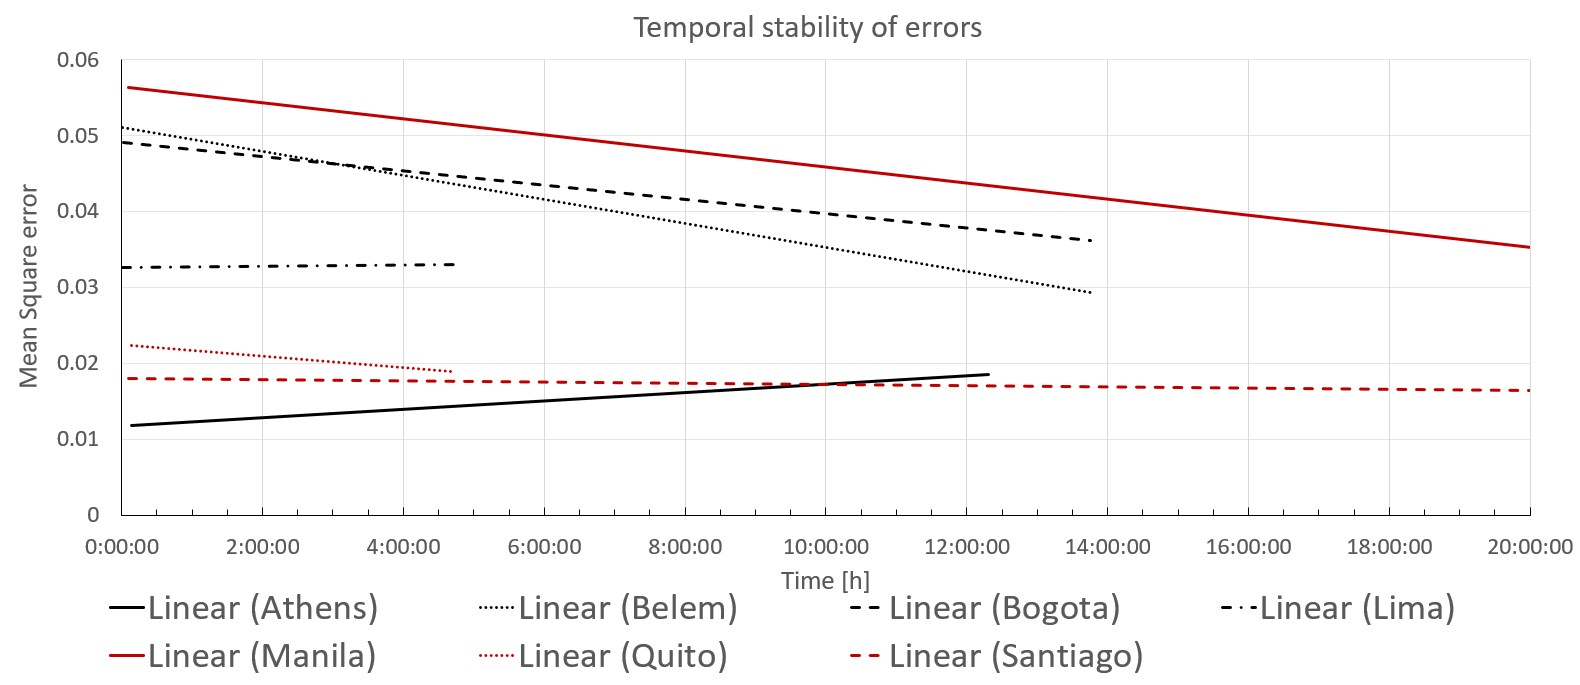
\includegraphics[width=\textwidth]{figures/chp_pdu/pdu_trend_iccs.jpg}
\caption{w funkcji czasu od kalibracji ustalającej błędy urządzenia~\cite{werner_experiment_driven_2022}}
\label{fig:pdu:trends:iccs}
\end{subfigure}

\smallskip
\begin{subfigure}{0.63\textwidth}
\centering
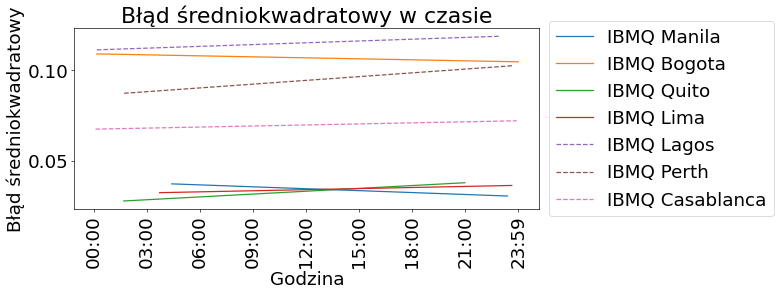
\includegraphics[width=\textwidth]{figures/chp_pdu/pdu_trend_msc.png}
\caption{w funkcji godziny doby~\cite{werner_magisterka_2022}}
\label{fig:pdu:trends:msc}
\end{subfigure}
\caption[Linie trendu błędu średniokwadratowego obwodu referencyjnego]{Linie trendu błędu średniokwadratowego wyników obwodu referencyjnego przed korektą, wyznaczone dla dwóch zbiorów danych: (a)~siedem urządzeń pięciokubitowych, (b)~urządzenia pięcio- i siedmiokubitowe.
Rysunki własne autora, przeniesione z~prac źródłowych bez zmian; na rysunku (a) oś pozioma to czas w~godzinach, a oś pionowa to błąd średniokwadratowy.}
\label{fig:pdu:trends}
\end{figure}

Linie trendu dają jedynie warunek konieczny stabilności: z nierówności trójkąta wynika, że zmiana błędu średniokwadratowego wyniku nieskorygowanego z wartości $\mathrm{MSE}_0$ do $\mathrm{MSE}_t$ ogranicza średni kwadrat dryfu tylko od dołu, $\langle\delta_t^2\rangle\ge\bigl(\sqrt{\mathrm{MSE}_t}-\sqrt{\mathrm{MSE}_0}\bigr)^2$; bezpośrednim oszacowaniem dryfu jest dopiero błąd po korekcie (podrozdział~\ref{subsec:pdu:results:one}).
% Usunięto przykład liczbowy (PHD-TS-91, ustalenia I5 i D15 recenzji): dla największej zmiany odczytanej z rysunku time stability.jpg (Belem, 0,0509 -> 0,0293 w 13,8 h) ograniczenie wynosi (sqrt(0.0509)-sqrt(0.0293))^2 = 0.0030, a dla urządzenia Manila (0.0563 -> 0.0353) 0.0024; wartości są orientacyjne, bo linie dopasowano do pomiarów z wielu dni, a ograniczenie dolne nie świadczy o stabilności.

\subsection{Korekta funkcji jednej zmiennej}\label{subsec:pdu:results:one}
\agentinfo{
Rysunek fig:pdu:example: cztery grafiki przeniesione z pracy magisterskiej (te same pliki są w katalogu artykułu): Quito, składnik o częstotliwości 2, zrzuty z 11.04.2022; Belem, MSE i odchylenie standardowe z 14.12.2021.
Wartości 0,0190, 0,0016, 0,1333 i 0,0401 podaje tylko artykuł (sekcja Results, słowa: in the cases shown there); po recenzji (ustalenie B2, PHD-TS-91) tekst przypisuje je artykułowi i podaje obok odczyt ze słupków rysunku (MSE 0,046 i 0,0005; odchylenie 0,21 i 0,02), który im nie odpowiada; krotność 12 i iloraz 8 procent usunięto.
Hipoteza recenzenta, niewpisana do tekstu: liczby artykułu są wartościami zbiorczymi dla urządzenia Quito (z r = 0,994 po korekcie wynika MSE około 0,0015 i odchylenie około 0,039).
Uwaga recenzenta do rozważenia przez autora, niewprowadzona: zbiorcze MSE po korekcie można oszacować pośrednio z wartości r po korekcie jako 0,125 razy (1/r^2 - 1), przy założeniu, że reszta nie jest skorelowana z wartością oczekiwaną (łącznie około 0,0033, od 0,0008 dla Limy do 0,0090 dla Belem); usunęłoby to lukę braku zbiorczych MSE.
Odczyt serii z urządzenia Belem (PHD-TS-91, skrypt recenzenta odczyt_serii.py): MSE przed korektą 0,029--0,062, po korekcie 0,006--0,015, iloraz 0,13--0,38 (mediana 0,25); oś czasu 33--162 minuty.
ROZBIEŻNOŚCI (DO DECYZJI AUTORA; w tekście zestawia je tabela tab:pdu:app:discrepancies w dodatku):
(1) dwa zbiory danych: artykuł ma 6006 próbek (tabela) albo 6005 (wykomentowany tekst: Belem 1248, Bogota 1857, Manila 1026, Quito 265), praca magisterska 10086; współczynniki Pearsona przed korektą różnią się (łącznie 0,876 wobec 0,761; Bogota 0,887 wobec 0,646);
(2) artykuł podaje przyrost dla Santiago 0.099, a plik pearson.png z katalogu artykułu 0.0099 (zgodne z wartościami 0.9785 i 0.99);
(3) praca magisterska podaje w tekście, że najmniejszy przyrost (0.0895) dotyczy urządzenia Manila, a z jej tabeli wynika 0.121 dla Manila i najmniejszy przyrost dla Athens (0.003), potem Quito (0.081);
(4) podpis rysunku z MSE i odchyleniem standardowym w artykule mówi o urządzeniu Lima i szeregu dwuskładnikowym, a włączone pliki pochodzą z urządzenia Belem (tak opisuje je praca magisterska);
(5) część rysunków przykładowych z czerwca 2022 r. ma oś argumentów opisaną od -2 pi do 3/2 pi (podwojone etykiety); tych rysunków nie przeniesiono.
Przedziały ufności w tabeli tab:pdu:corr obliczono w rozprawie przekształceniem Fishera z wartości r i N podanych w pracy magisterskiej.
Wykres fig:pdu:pearson (wartości r z tabel tab:pdu:corr i tab:pdu:app:iccs) przeniesiono w zadaniu PHD-TS-97 do dodatku, sekcja app:results:pdu2.
}

\begin{figure}[tb]
\centering
\begin{tabular}{@{}cc@{}}
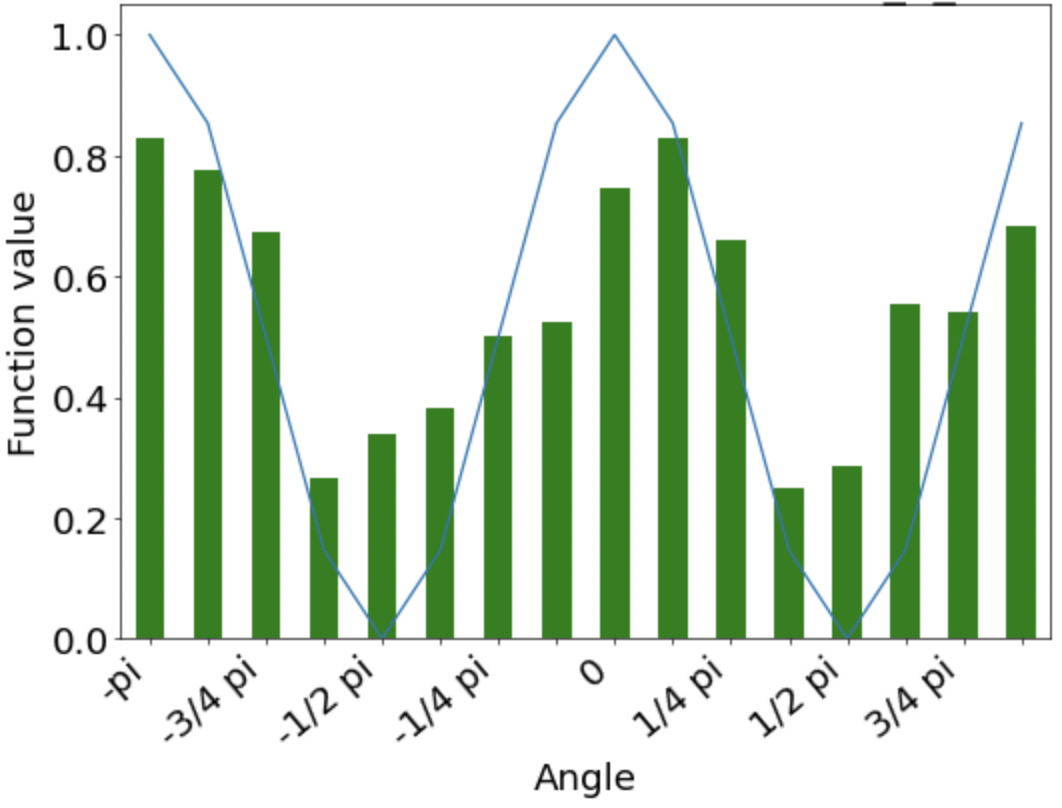
\includegraphics[width=0.30\textwidth]{figures/chp_pdu/pdu_quito_cos2x_before.png} &
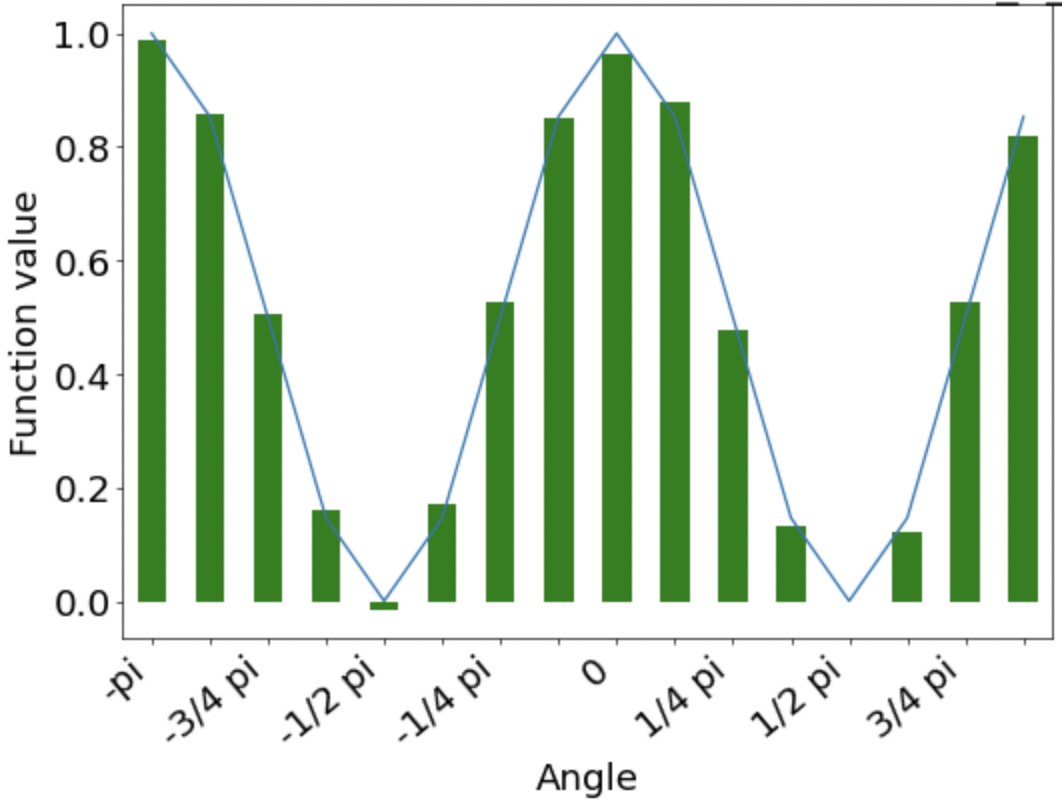
\includegraphics[width=0.30\textwidth]{figures/chp_pdu/pdu_quito_cos2x_after.png} \\
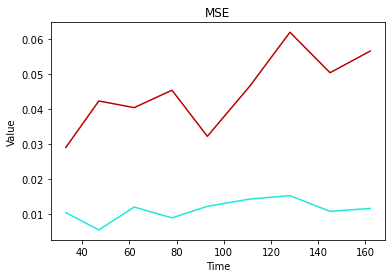
\includegraphics[width=0.30\textwidth]{figures/chp_pdu/pdu_belem_mse.png} &
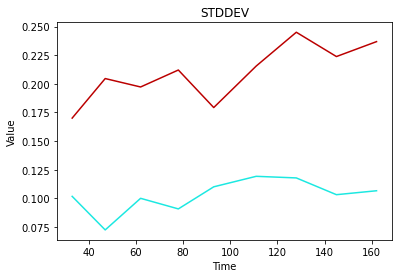
\includegraphics[width=0.30\textwidth]{figures/chp_pdu/pdu_belem_stddev.png}
\end{tabular}
\caption[Przykład korekty funkcją PDU na urządzeniach Quito i Belem]{Górny wiersz: wartości składnika $\coscomp_{2,0}$ uzyskane na urządzeniu Quito (słupki) na tle wartości oczekiwanych (linia), przed korektą (po lewej) i po korekcie (po prawej).
Dolny wiersz: błąd średniokwadratowy (po lewej) i odchylenie standardowe błędu (po prawej) kolejnych serii na urządzeniu Belem w~funkcji czasu od kalibracji funkcji PDU w~minutach; linia czerwona oznacza wynik przed korektą, linia turkusowa po korekcie.
Rysunki własne autora, przeniesione z~prac~\cite{werner_experiment_driven_2022,werner_magisterka_2022}.}
\label{fig:pdu:example}
\end{figure}

Działanie korekty na pojedynczym wyniku pokazuje górny wiersz rysunku~\ref{fig:pdu:example}: wartości składnika $\coscomp_{2,0}$ uzyskane na urządzeniu Quito 20~godzin po kalibracji urządzenia~\cite{werner_magisterka_2022}; czasu od kalibracji funkcji PDU źródła nie podają.
Praca~\cite{werner_experiment_driven_2022} podaje przy tym rysunku spadek błędu średniokwadratowego z $0{,}0190$ do $0{,}0016$ i odchylenia standardowego błędu z $0{,}1333$ do $0{,}0401$, ale odczyt wysokości słupków (dokładność około $0{,}002$) daje dla pokazanej serii MSE około $0{,}046$ przed korektą i $0{,}0005$ po niej; przy obu parach liczb błąd średniokwadratowy maleje ponad dziesięciokrotnie.
% ŹRÓDŁO: ICCS main.tex, sekcja Results, akapit ,,Significance of the PDU method'' (in the cases shown there); 20 godzin: magisterka 03.tex, opis rysunku fig:corrections_q.
% ŹRÓDŁO: odczyt z plików rozprawa/figures/chp_pdu/pdu_quito_cos2x_before.png i pdu_quito_cos2x_after.png skryptem eksperymenty/recenzje/_robocze/PHD-TS-62/odczyt_rysunkow.py (powtórzony w PHD-TS-91, plik powt_odczyt_rysunkow.txt): MSE 0,0459 i 0,0005; odchylenie standardowe błędu 0,2084 i 0,0204; rozdzielczość 0,0017--0,0018 na piksel; niezależny odczyt wzrokowy w PHD-TS-91 daje MSE przed korektą 0,046.
\agenttask{
Pytanie do autora (recenzja rozdziału 4, ustalenie B2): do której serii albo do jakiego zbioru odnoszą się wartości 0,0190, 0,0016, 0,1333 i 0,0401 z artykułu ICCS (pojedyncza seria z rysunku czy wartości zbiorcze dla urządzenia Quito) oraz ile czasu upłynęło między kalibracją funkcji PDU a serią pokazaną na rysunku?
Słupki na rysunku dają MSE około 0,046 przed korektą i 0,0005 po korekcie, więc liczby artykułu nie opisują pokazanej serii.
}%
Dolny wiersz przedstawia MSE i $\sigma_e$ dziewięciu kolejnych serii na urządzeniu Belem, od 33 do 162~minut po kalibracji funkcji PDU: według odczytu z rysunku błąd średniokwadratowy po korekcie stanowił od $13\%$ do $38\%$ błędu przed korektą.
% ŹRÓDŁO: odczyt z pliku rozprawa/figures/chp_pdu/pdu_belem_mse.png skryptem eksperymenty/recenzje/_robocze/PHD-TS-62/odczyt_serii.py (powtórzony w PHD-TS-91, plik powt_odczyt_serii.txt) w dziewięciu wierzchołkach linii (33, 47, 62, 78, 93, 111, 128, 145 i 162 min): przed korektą 0,029--0,062, po korekcie 0,0057--0,0154 (0,006--0,012 w pierwszych pięciu seriach, 0,011--0,015 w czterech ostatnich); ilorazy 0,13--0,38, mediana 0,25.
Ponieważ węzły kalibracji i węzły korygowanych wyników pokrywają się, wynik skorygowany jest tu sumą wartości oczekiwanej i różnicy dwóch pomiarów, korygowanego i kalibracyjnego.
Miary po korekcie oceniają zatem powtarzalność błędu między tymi pomiarami, a zgodnie ze wzorem~\eqref{eq:pdu:residual} błąd średniokwadratowy po korekcie jest bezpośrednim oszacowaniem średniego kwadratu dryfu.
Już w pierwszej serii, pół godziny po kalibracji, przekracza on granicę próbkowania $2/(4\nshots)\approx 6\cdot10^{-5}$ o dwa rzędy wielkości, więc dryf zawiera składową zmienną między kolejnymi seriami, a warunek~\eqref{eq:pdu:stability} jest spełniony tylko w słabym sensie kilkakrotnego zmniejszenia błędu.
% ŹRÓDŁO: obliczenie własne: 2/(4*8192) = 6,1e-5; MSE po korekcie w pierwszej serii około 0,010 (odczyt jak wyżej).

\begin{table}[tb]
\centering
\caption[Współczynniki korelacji wyników z wartościami oczekiwanymi przed korektą i po korekcie funkcją PDU]{Współczynniki korelacji wyników z wartościami oczekiwanymi przed korektą i po korekcie funkcją PDU: $r$ Pearsona z $95$-procentowym przedziałem ufności, $\tau$ Kendalla i $r_{\mathrm{S}}$ Spearmana; $N$ oznacza liczbę próbek.
Współczynniki i liczności według~\cite{werner_magisterka_2022}, przedziały ufności obliczone w rozprawie.}
\label{tab:pdu:corr}
\footnotesize
\begin{tabular}{@{}lrcccccc@{}}
\toprule
 & & \multicolumn{2}{c}{$r$ [95\% PU]} & \multicolumn{2}{c}{$\tau$} & \multicolumn{2}{c}{$r_{\mathrm{S}}$} \\
\cmidrule(lr){3-4}\cmidrule(lr){5-6}\cmidrule(l){7-8}
\textbf{Urządzenie} & $N$ & przed & po & przed & po & przed & po \\
\midrule
\multicolumn{8}{@{}l}{\emph{Funkcje jednej zmiennej (E3), urządzenia pięciokubitowe}} \\
Athens & 100 & 0,978 [0,967; 0,985] & 0,981 [0,972; 0,987] & 0,886 & 0,913 & 0,973 & 0,982 \\
Belem & 1248 & 0,836 [0,818; 0,852] & 0,966 [0,962; 0,970] & 0,653 & 0,843 & 0,828 & 0,956 \\
Bogota & 3760 & 0,646 [0,627; 0,664] & 0,978 [0,977; 0,979] & 0,516 & 0,866 & 0,649 & 0,968 \\
Lima & 1470 & 0,892 [0,881; 0,902] & 0,997 [0,997; 0,997] & 0,735 & 0,873 & 0,892 & 0,968 \\
Manila & 1667 & 0,855 [0,842; 0,867] & 0,976 [0,974; 0,978] & 0,693 & 0,874 & 0,852 & 0,969 \\
Quito & 1162 & 0,913 [0,903; 0,922] & 0,994 [0,993; 0,995] & 0,737 & 0,915 & 0,895 & 0,986 \\
Santiago & 679 & 0,875 [0,856; 0,892] & 0,990 [0,988; 0,991] & 0,737 & 0,901 & 0,866 & 0,982 \\
łącznie & 10\,086 & 0,761 [0,753; 0,769] & 0,987 [0,986; 0,987] & 0,580 & 0,900 & 0,741 & 0,979 \\
\midrule
\multicolumn{8}{@{}l}{\emph{Funkcja dwóch zmiennych (E5), urządzenia siedmiokubitowe}} \\
Casablanca & 5056 & 0,691 [0,676; 0,705] & 0,522 [0,502; 0,542] & 0,471 & 0,340 & 0,649 & 0,469 \\
Jakarta & 6208 & 0,506 [0,487; 0,524] & 0,363 [0,341; 0,384] & 0,384 & 0,328 & 0,532 & 0,457 \\
Lagos & 6272 & 0,378 [0,357; 0,399] & 0,355 [0,333; 0,376] & 0,239 & 0,236 & 0,343 & 0,331 \\
Perth & 4224 & 0,525 [0,503; 0,547] & 0,491 [0,468; 0,514] & 0,335 & 0,327 & 0,488 & 0,468 \\
łącznie & 21\,760 & 0,507 [0,497; 0,517] & 0,418 [0,407; 0,429] & 0,344 & 0,302 & 0,488 & 0,423 \\
\bottomrule
\end{tabular}
\end{table}
% ŹRÓDŁO tabeli: artykuły/magisterka_werner_final/chapters/03.tex, tabele tab:pearson_coefficients, tab:other_corrs_tau, tab:other_corrs_rho (E3) oraz tab:pearson_coefficients_seven, tab:other_corrs_seven (E5) i zdania z wartościami łącznymi; przedziały ufności: tanh(artanh(r) +/- 1,96/sqrt(N-3)).

W skali całego zbioru danych współczynniki korelacji wyników z wartościami oczekiwanymi wzrosły po korekcie na każdym urządzeniu (tabela~\ref{tab:pdu:corr}; rysunek~\ref{fig:pdu:pearson} w dodatku).
W zbiorze z pracy magisterskiej, liczącym $10\,086$ próbek, współczynnik Pearsona wzrósł z $0{,}761$ do $0{,}987$~\cite{werner_magisterka_2022}, a w mniejszym zbiorze opisanym w artykule ($6006$ próbek) z $0{,}876$ do $0{,}971$~\cite{werner_experiment_driven_2022}.
% ŹRÓDŁO: magisterka 03.tex, tabela tab:pearson_coefficients i zdanie pod nią; ICCS main.tex, sekcja Results (0.876, 0.9707) i tabela tab:coefficients (liczności; suma 6006 to obliczenie własne, w tekście artykułu nie pada).
Oba zbiory różnią się licznością i, poza urządzeniami Athens i Belem, wartościami współczynników przed korektą, zgodnie natomiast dają po korekcie wartości od $0{,}96$ do $1{,}00$.
Przedziały ufności współczynnika $r$ przed korektą i po korekcie są rozłączne dla wszystkich urządzeń z wyjątkiem Athens, także przy liczbie jednostek równej liczbie serii; dla urządzenia Athens zebrano tylko $100$ próbek, a korelacja już przed korektą wynosiła $0{,}978$, więc poprawy nie można uznać za wykazaną~\cite{werner_magisterka_2022}.
% ŹRÓDŁO: obliczenie własne z wartości r i N z tabeli tab:pdu:corr: tanh(artanh(r) +/- 1,96/sqrt(n-3)) dla n = N oraz n = N/16 (część całkowita); skrypt eksperymenty/recenzje/_robocze/PHD-TS-62/analiza_wrazliwosci.py, wynik powtórzony w PHD-TS-91 (plik powt_analiza_wrazliwosci.txt).
P-wartości oraz wyniki dla zbioru z artykułu zawiera dodatek (strona~\pageref{tab:pdu:app:pvalues}).
Według pracy~\cite{werner_magisterka_2022} funkcja PDU zmniejszała błąd nawet wiele godzin po kalibracji, do najbliższej kalibracji ustalającej nowe błędy urządzenia; źródło nie podaje przy tym liczb, a przykłady z osią czasu obejmują niespełna trzy godziny.
% ŹRÓDŁO: magisterka 03.tex, sekcja ,,Korekcja funkcji jednej zmiennej'', podsekcja ,,Wyniki eksperymentu'' (funkcja PDU skutecznie redukuje błąd nawet wiele godzin po kalibracji, dopóki nie nastąpiła kalibracja ustalająca nowe błędy); osie czasu rysunków fig:pdu:example (33--162 min) i fig:pdu:two-comp (18--94 min), odczyt skryptem odczyt_serii.py.
Dla badanych urządzeń pięciokubitowych odpowiedź na pytanie PB1 jest zatem twierdząca tylko w postaci słabszej, omówionej w podrozdziale~\ref{sec:pdu:discussion}.

\subsection{Korekta funkcji dwóch zmiennych i szeregów wieloskładnikowych}\label{subsec:pdu:results:two}
\agentinfo{
Rysunek fig:pdu:two-comp (od zadania PHD-TS-97 w dodatku, sekcja app:results:pdu2, razem z komentarzem źródłowym do dat w podpisie): trzy grafiki przeniesione z pracy magisterskiej (katalog wiele_komp; daty w nazwach plików 19.06.2022 i 19.01.2022); poziomy MSE (0,06--0,09 oraz poniżej 0,005) odczytano z osi wykresu, źródła nie podają dla tego eksperymentu statystyk zbiorczych ani sposobu kalibracji.
Wyniki eksperymentu dwóch zmiennych pochodzą wyłącznie z pracy magisterskiej (tabele tab:pearson_coefficients_seven i tab:other_corrs_seven); artykuł ich nie zawiera.
Rysunków z katalogu dwie_zmienne nie przeniesiono, bo praca magisterska ich nie opisuje i nie da się ustalić znaczenia serii.
Interpretacje dodane w rozprawie, DO AKCEPTACJI AUTORA: podwójne liczenie wspólnej części błędu przy sumowaniu poprawek oraz (po recenzji, ustalenie I7) uwaga, że sumowanie poprawek nie jest zastosowaniem definicji def:pdu:correction i że w modelu eq:tb:noise:fringe suma poprawek dla x i y nie jest poprawką dla x+y; praca magisterska mówi o pominiętym oddziaływaniu rejestrów i o możliwym współczynniku wagowym.
Recenzent policzył ilustrację liczbową tej uwagi (dla widoczności 0,7 i zerowego przesunięcia fazy korelacja spada po dodaniu sumy poprawek z 1,00 do 0,86); zgodnie z jego zaleceniem nie wprowadzono jej do tekstu bez decyzji autora.
Po recenzji (ustalenia I1, I2 i I6, PHD-TS-91): wniosek dla PB2 brzmi, że korekta poprawia wyniki obwodów, na których ją wyznaczono, a przenoszenia z funkcji referencyjnej na inne funkcje nie da się na podstawie źródeł potwierdzić; eksperyment E5 nazwano sprawdzeniem addytywności poprawek, a nie założenia Z8; dla E5 odporny jest wniosek o braku poprawy, nie o pogorszeniu (przedziały liczone dla serii zachodzą na siebie).
Odczyt słupków z rysunku fig:pdu:two-comp: przed korektą MSE 0,087 i korelacja z wartościami oczekiwanymi -0,53, po korekcie 0,0037 i +0,97.
Nazwa pliku z przebiegiem MSE na tym rysunku kończy się na MSE_cos_phi i ma datę 19.01.2022, a słupki pochodzą z 19.06.2022; praca magisterska opisuje przebieg jako wynik dla operatora wieloskładnikowego (pytanie do autora w zadaniu na końcu sekcji).
Zdanie proponujące powtórzenie eksperymentu w dwóch wariantach usunięto z tekstu (zasada: rozdział nie proponuje nowych eksperymentów); wcześniejsza propozycja z tego konspektu (E3 w dwóch wariantach kalibracji i E5 z pełną kalibracją na 64 obwodach, na symulatorze) pozostaje do decyzji autora i jest odłożona zgodnie z CLAUDE.md.
}

Dla szeregu dwuskładnikowego $\tfrac{1}{2}(\coscomp_{1,0}+\coscomp_{2,0})$, badanego na urządzeniu Lima (eksperyment E4), błąd średniokwadratowy kolejnych serii maleje po korekcie z poziomu $0{,}06$--$0{,}09$ do wartości poniżej $0{,}005$ (rysunek~\ref{fig:pdu:two-comp} w dodatku).
% ŹRÓDŁO: odczyt z rysunków wiele_komp/result_2_..., correctedResult_2_... i 01_19_2022_02_27_24_ibmq_lima_MSE_cos_phi.png (magisterka).
W pokazanej serii wynik nieskorygowany nie odtwarza jednak funkcji (odczyt ze słupków: korelacja z wartościami oczekiwanymi około $-0{,}5$ przed korektą i $0{,}97$ po korekcie), więc kształt widoczny po korekcie wnosi poprawka, a nie pomiar.
% ŹRÓDŁO: odczyt z plików rozprawa/figures/chp_pdu/pdu_lima_two_comp_before.png i pdu_lima_two_comp_after.png skryptem eksperymenty/recenzje/_robocze/PHD-TS-62/odczyt_rysunkow.py (powtórzony w PHD-TS-91, plik powt_odczyt_rysunkow.txt): r = -0,525 i +0,972; MSE 0,0866 i 0,0037 (osiem węzłów).
Sposobu kalibracji ani statystyk zbiorczych źródła nie podają, więc wynik ma charakter jakościowy i nie dowodzi przenoszenia korekty z funkcji referencyjnej.

Eksperyment E5 dał wynik negatywny.
Po korekcie sumą błędów obu rejestrów współczynniki korelacji zmalały na wszystkich czterech urządzeniach (tabela~\ref{tab:pdu:corr}): w zbiorze $21\,760$ próbek współczynnik Pearsona spadł z $0{,}507$ do $0{,}418$~\cite{werner_magisterka_2022}.
% ŹRÓDŁO: magisterka 03.tex, sekcja ,,Korekcja funkcji dwóch zmiennych'', podsekcja ,,Wyniki eksperymentu''.
Przedziały ufności liczone dla próbek są rozłączne dla zbioru łącznego oraz dla urządzeń Casablanca i Jakarta, a liczone dla serii zachodzą na siebie w każdym przypadku, więc odporny jest wniosek o braku poprawy, a nie o pogorszeniu.
% ŹRÓDŁO: obliczenie własne z wartości r i N z tabeli tab:pdu:corr dla n = N/64: łącznie n = 340, r = 0,507: [0,423; 0,582]; r = 0,418: [0,326; 0,502]; Casablanca (n = 79): [0,555; 0,791] i [0,340; 0,666]; Jakarta (n = 97): [0,341; 0,641] i [0,176; 0,524]; skrypt eksperymenty/recenzje/_robocze/PHD-TS-62/analiza_wrazliwosci.py, wynik powtórzony w PHD-TS-91.
Za prawdopodobną przyczynę uznano sposób kalibracji: błędy wyznaczone osobno dla każdego rejestru nie obejmowały oddziaływania rejestrów ani bramek drugiego rejestru~\cite{werner_magisterka_2022}.
Sumowanie poprawek nie jest ponadto zastosowaniem definicji~\ref{def:pdu:correction}, która wymagałaby funkcji PDU odczytanej dla fazy łącznej $x+y$: już w modelu~\eqref{eq:tb:noise:fringe} suma poprawek dla $x$ i $y$ nie jest na ogół poprawką dla $x+y$, a błąd odczytu, wspólny dla obu kalibracji, jest liczony dwukrotnie.
Żadnego z tych wyjaśnień nie sprawdzono: kalibracji na obwodach zawierających bramki obu rejestrów, w granicznym przypadku na wszystkich $64$ konfiguracjach, nie przeprowadzono.

Odpowiedź na pytanie PB2 jest zatem warunkowa, przy czym eksperyment E5 sprawdza inną hipotezę niż założenie~(\ref{itm:pdu:Z8}): addytywność poprawek rejestrów.
Korekta poprawia wyniki obwodów, na których ją wyznaczono, i nie przenosi się przez składanie poprawek wyznaczonych dla części układu; przenoszenia z funkcji referencyjnej na inne funkcje źródła nie pozwalają potwierdzić.
Praca~\cite{werner_experiment_driven_2022} opisuje wprawdzie korektę składnika $\coscomp_{2,0}$ funkcją wyznaczoną na funkcji referencyjnej, ale na rysunku~\ref{fig:pdu:example} poprawki w węzłach $x$ i $x+\pi$, o tej samej fazie $2x$ kubitu odczytu, różnią się nawet o $0{,}22$ (odczyt ze słupków).
% ŹRÓDŁO: odczyt jak w podrozdziale subsec:pdu:results:one (skrypt odczyt_rysunkow.py, plik powt_odczyt_rysunkow.txt): poprawka (wynik po korekcie minus przed korektą) w węzłach -3/8 pi i 5/8 pi: -0,209 i -0,431; w węzłach -1/8 pi i 7/8 pi: +0,321 i +0,136; błąd przed korektą w tych parach: +0,233 i +0,406 oraz -0,331 i -0,172; średnia kwadratowa różnic poprawek w ośmiu parach 0,109; niezależny odczyt wzrokowy w PHD-TS-91: -0,215 i -0,435 oraz +0,325 i +0,135.
Jeżeli oba panele pokazują tę samą serię, to przykład jest zgodny z tablicą wyznaczoną na obwodach korygowanego składnika, opisaną w pracy~\cite{werner_magisterka_2022}, i niezgodny z poprawką odczytywaną według samej fazy.
Wyznaczanie korekty raz dla rodziny obwodów jest więc potwierdzone dla obwodów jednej funkcji różniących się konfiguracją wejścia.
\agenttask{
Pytanie do autora (recenzja rozdziału 4, ustalenia I1 i I2): na jakich obwodach wyznaczano tablicę błędów użytą do korekty składnika o częstotliwości 2 (eksperyment E3) i szeregu dwuskładnikowego (eksperyment E4): na obwodach funkcji referencyjnej cos x, z odczytem poprawki dla fazy 2x, czy na tych samych obwodach, które potem korygowano?
Odczyt rysunku fig:pdu:example wskazuje drugi wariant (poprawki w węzłach o tej samej fazie różnią się nawet o 0,22), ale to jeden przykład i odczyt z rysunku rastrowego; po odpowiedzi doprecyzować wniosek dla PB2, zakres pierwszego wyróżnika metody w sekcjach 4.8 i 4.9 oraz brzmienie założenia Z8.
Dodatkowa obserwacja do tego samego pytania: nazwa pliku z przebiegiem MSE na rysunku fig:pdu:two-comp kończy się na MSE_cos_phi i ma datę 19.01.2022, a słupki pochodzą z 19.06.2022; czy ten przebieg dotyczy szeregu dwuskładnikowego?
}

\section{Dyskusja}\label{sec:pdu:discussion}
\agentinfo{
Napisane w zadaniu PHD-TS-57 (2026-11-27) z wyników sekcji 4.7 oraz z sekcji 3.3 i 3.5 i podrozdziału 2.3; bez nowych liczb i bez nowych pozycji bibliograficznych.
Decyzje autora z 2026-11-27: PDU jest metodą rozwijaną w ramach tego doktoratu i ważnym wkładem rozprawy; jej wyróżnikami względem metod pokrewnych są korekta indeksowana znanym argumentem, wyznaczana raz dla rodziny obwodów, oraz zbadanie stabilności błędu między kalibracjami urządzenia; metody pokrewne trzeba przywoływać (sekcja 3.3) i nie wolno pisać, że ich nie ma ani że PDU jest pierwsza.
Pytania rozdziału opisano słownie, bez numerów i bez brzmienia tezy (numeracja niezatwierdzona, zadanie pod akapitem).
Zgodnie z decyzją autora tekst nie proponuje nowych eksperymentów ani kierunków badań; mówi tylko, czego dane nie rozstrzygają.
Oceny własne, a nie twierdzenia cytowanych prac (DO AKCEPTACJI AUTORA): odczytanie wyników sekcji 4.7 jako potwierdzenia słabszej postaci założenia Z4; uwaga, że linia trendu może nie wykryć zmian skokowych; uwaga, że deklarowana kalibracja urządzenia wyznacza najwyżej górną granicę ważności funkcji PDU; zdanie o ponownym pomiarze węzłów jako sposobie rozpoznania nieaktualnej funkcji PDU (pomysł z konspektu sekcji 4.5, w eksperymentach niestosowany; to uwaga o regule ponownej kalibracji, nie propozycja badań).
Obserwacje o częstości kalibracji procesorów IBM pochodzą z sekcji 3.5: wilson_just-in-time_2020 dotyczy innych urządzeń i lat 2019--2020, a etxezarreta_multiqubit_2023 (dodatek C) tych samych procesorów pięciokubitowych (santiago i bogota kilka kalibracji na dobę; quito, belem i lima około jednej); roku tych pomiarów praca nie podaje (według notatki do sekcji 3.5 daty kwietniowe, preprint z lipca 2022), więc nie można wykluczyć, że pokrywają się z okresem eksperymentów PDU; dlatego tekst nie twierdzi, że pochodzą z innych dat.
Hipotezy o związku rozrzutu na urządzeniu Santiago z częstszymi kalibracjami nie wpisano (zadanie w sekcji 3.5).
Dopisane w zadaniu PHD-TS-94 (2026-11-27, po decyzji autora, że dawny rozdział 9 o strukturze szumu nie jest osobnym rozdziałem): trzy zdania na końcu akapitu o założeniu Z4, odnoszące się do pracy raubitzek_quantum_noise omawianej w sekcji 3.5 (akapit par:lr:noise:generators); praca jest pracą powiązaną z udziałem autora, a nie wkładem rozprawy.
Oceny własne w tych zdaniach (DO AKCEPTACJI AUTORA): warunek stabilności zaburzeń w schemacie z tej pracy jest odpowiednikiem założenia Z4; praca nie rozstrzyga o stałości błędu między kalibracjami; opis na poziomie generatorów jest uzupełnieniem, a nie uzasadnieniem metody PDU.
Zdania nie korzystają z elementów macierzy, których dotyczy ustalenie B1 recenzji dawnego rozdziału 9 \agentref{eksperymenty/recenzje/rozdzial-9.md}.
Zdanie, że rozdział opiera się na tekście, tabelach i rysunkach prac źródłowych, a nie na danych pierwotnych, zmienić, gdy autor dostarczy oryginalne dane eksperymentów PDU.
Pominięto dla objętości: osobne zdanie o mitygacji błędu odczytu (jest w podrozdziale 2.3 i w tabeli tab:lr:qem:calibrated); użyteczność metody poza erą NISQ (wstęp artykułu ICCS nazywa ją problematyczną); obserwację z wniosków artykułu ICCS, że urządzenia o bardziej poziomej linii trendu nie miały większego przyrostu korelacji; to, że zbiór z artykułu nie jest podzbiorem zbioru z pracy magisterskiej (dla urządzenia Belem tabela artykułu podaje 1360 próbek, a praca magisterska 1248; por. tabele tab:pdu:corr i tab:pdu:app:iccs); rozbieżności szczegółów protokołu opisane w konspekcie sekcji 4.6; zastrzeżenie, że poprawy dla urządzenia Athens nie wykazano (jest w sekcji 4.7.3).
Po recenzji (PHD-TS-91) uzgodniono dyskusję z poprawionymi sekcjami 4.4--4.7: odpowiedź o stabilności jest twierdząca w postaci słabszej (linie trendu nie pozwalają stwierdzić ani narastania błędu, ani jego stałości; korekta wyznaczona raz zwiększała zgodność wyników w badanych seriach), odpowiedź o przenoszeniu mówi, że korekta poprawia wyniki obwodów, na których ją wyznaczono, a przenoszenia między funkcjami źródła nie pozwalają potwierdzić; przy pierwszym wyróżniku podano zakres potwierdzenia (obwody jednej funkcji różniące się konfiguracją wejścia); usunięto słowa o poprawie przez wiele godzin i o braku wyraźnego trendu; dodano zdanie o nieudokumentowanej kontroli układu kubitów i transpilacji; trzy zdania podzielono.
Skróty z zadań PHD-TS-91 i PHD-TS-97 (wykazy w plikach wskazanych w konspekcie rozdziału): w dyskusji nie powtarza się zdania o przedziałach ufności, wyliczenia rozbieżności źródeł, zdania o wycofanych urządzeniach, wniosku o składaniu poprawek z eksperymentu E5 ani odesłania do wykresu współczynników korelacji; trzy zdania o pracy o zaburzeniach generatorów ściśnięto bez zmiany treści.
Objętość (kompilacja bez notatek, 2026-11-28, po przywróceniu schematu blokowego): treść zajmuje 16 stron i 6 wierszy na siedemnastej, w spisie treści rozdział ma 18 stron (rozdziały zaczynają się na stronie nieparzystej).
Decyzja autora z 2026-11-28: zostawić 17 stron, nie skracać rozdziału o te 6 wierszy.
Każde dalsze dopisanie zdania albo przywrócenie rysunku z dodatku wydłuża siedemnastą stronę; przekroczenie jej wymaga cięcia o tej samej wielkości.
}

W kategoriach kryteriów K1--K6 (tabela~\ref{tab:tb03:cost}) PDU nie zużywa dodatkowych kubitów ani bramek, a płaci wykonaniami obwodów kalibracyjnych (K3), założeniem o powtarzalności błędu (K5) i wąskim zakresem stosowalności metody zorientowanej na problem (K6); korekcji nie zastępuje, bo usuwa jedynie powtarzalną część błędu wyniku.
Samo to położenie nie wyróżnia jednak PDU: korektę wyznaczaną na obwodach o znanym wyniku i stosowaną klasycznie do wyniku niezmienionego obwodu zadania opisywano od 2020~r.~\cite{jattana_general_2020,czarnik_error_2021,urbanek_mitigating_2021,lolur_reference-state_2023}, a PDU jest własną realizacją tej zasady (podrozdział~\ref{sec:lr:qem}, tabela~\ref{tab:lr:qem:calibrated}).
Od metod tych odróżniają ją dwie cechy.
Po pierwsze, korekta jest tablicą błędów indeksowaną znanym argumentem, a nie funkcją wartości zmierzonej, i wyznacza się ją raz dla rodziny obwodów w każdym okresie między kalibracjami urządzenia, a nie osobno dla każdego obwodu zadania; w danych tego rozdziału rodzinę tę tworzą obwody jednej funkcji różniące się konfiguracją wejścia.
Samo wyznaczanie korekty raz dla obwodów o stałej strukturze ma odpowiednik w preprincie z 2025~r.~\cite{shen_circuit_2025}, więc odrębne dla PDU pozostaje w tej cesze indeksowanie znanym argumentem (podrozdział~\ref{sec:lr:qem}).
Po drugie, zbadano stabilność błędu między kalibracjami urządzenia (eksperymenty E2 i E3), a w tekstach głównych tamtych prac takich badań nie znaleziono.
Skalą demonstracji PDU nie wykracza natomiast poza prace pokrewne, a ceną pierwszej cechy jest wymóg znajomości argumentu (założenie~\ref{itm:pdu:Z7}): gdy argument nie jest znany, cecha ta nie ma zastosowania.

Na pytanie o stabilność błędu (podrozdział~\ref{sec:pdu:scope}) wyniki dają w zakresie badanych urządzeń pięciokubitowych odpowiedź twierdzącą w postaci słabszej: linie trendu nie pozwalają stwierdzić ani narastania błędu, ani jego stałości (rysunek~\ref{fig:pdu:trends}), a korekta wyznaczona raz zwiększała w badanych seriach zgodność wyników z wartościami oczekiwanymi, w obu zbiorach danych (tabela~\ref{tab:pdu:corr}).
Warunek~\eqref{eq:pdu:stability} sprawdzono bezpośrednio tylko w pojedynczych przykładach, do niespełna trzech godzin od kalibracji funkcji PDU (rysunek~\ref{fig:pdu:example}): zbiorczych wartości błędu średniokwadratowego po korekcie źródła nie podają, a współczynnik korelacji ocenia zgodność kształtu, nie wartości; dla urządzeń siedmiokubitowych dostępne są wyłącznie linie trendu.
Odpowiedź na pytanie o przenoszenie korekty pozostaje warunkowa (podrozdział~\ref{subsec:pdu:results:two}): korekta poprawia wyniki obwodów, na których ją wyznaczono, a tego, czy przenosi się między funkcjami, czyli jak szeroką rodzinę obwodów obsługuje jedna kalibracja, źródła nie pozwalają potwierdzić.
\agenttask{
Po zatwierdzeniu przez autora tez i numeracji pytań badawczych (sekcja sec:introduction:theses) dopisać w tym akapicie i w podsumowaniu rozdziału numery pytań, na które rozdział odpowiada (roboczo PB1 i PB2, tak jak w sekcjach 4.1, 4.2, 4.6 i 4.7), oraz zdanie odnoszące wyniki do tezy o redukcji błędów opartej na pomiarze (roboczo T1); do tego czasu nie przytaczać brzmienia tezy.
Uwaga orkiestratora do rozważenia przez autora (to nie jest decyzja): tezę T1 w brzmieniu ogólnym warto zawęzić do zakresu zbadanego w tym rozdziale.
}

Przegląd literatury w podrozdziale~\ref{sec:lr:noise} nie potwierdza założenia~(\ref{itm:pdu:Z4}) w postaci mocnej, czyli stałości błędu do następnej kalibracji urządzenia; zgodny jest z postacią słabszą, w której korekta wyznaczona z pomiaru zachowuje ważność przez czas rzędu godzin.
Wnioski te są pośrednie, bo przytoczone prace mierzą niemal wyłącznie parametry składowe, a nie błąd wyniku obwodu (tabela~\ref{tab:lr:noise:time}).
Zmiany tych parametrów bywają skokowe~\cite{klimov_fluctuations_2018,burnett_decoherence_2019}, a linia trendu, dopasowana do pomiarów z wielu okresów kalibracji, opisuje średnią zależność błędu od czasu, więc zmian epizodycznych w pojedynczym okresie nie wykrywa.
Czas od kalibracji jest ponadto wielkością deklarowaną przez dostawcę, a według innych prac częstość kalibracji procesorów IBM, także użytych w tym rozdziale, nie była stała i różniła się między urządzeniami~\cite{wilson_just-in-time_2020,etxezarreta_multiqubit_2023}, więc nie można przyjąć, że kalibracja była zawsze jednym zdarzeniem na dobę.
Wyniki podrozdziału~\ref{sec:pdu:results} należy zatem czytać jako stwierdzenie, że w badanych seriach korekta pozostawała korzystna, a nie jako dowód stałości błędu w całym okresie między kalibracjami.
Reguła ponownej kalibracji (podrozdział~\ref{sec:pdu:procedure}) wyznacza tym samym najwyżej górną granicę ważności funkcji PDU: warunek sprawdzany w algorytmie~\ref{alg:pdu:correction} jest konieczny, lecz niewystarczający.
Nieaktualna funkcja PDU, niespełniająca warunku~\eqref{eq:pdu:criterion}, może błąd zwiększać, a rozpoznać to pozwala dopiero ponowny pomiar węzłów, którego w eksperymentach nie stosowano.
Odpowiednikiem założenia~(\ref{itm:pdu:Z4}) jest warunek stabilności zaburzeń w schemacie diagnostycznym pracy o zaburzeniach generatorów bramek~\cite{raubitzek_quantum_noise} (podrozdział~\ref{par:lr:noise:generators}).
Praca ta nie rozstrzyga o stałości błędu między kalibracjami: zaburzenia dopasowano w niej do średniej z przebiegów zbieranych przez kilka miesięcy, nie rozdzielając rozrzutu między przebiegami na próbkowanie, dryf i zmiany kalibracji.
% ŹRÓDŁO: raubitzek_quantum_noise, wersja opublikowana (eksperymenty/_build/PHD-TS-38/work/pub/published.txt), sekcja VI.B, zastrzeżenie (2) (warunek stabilności), sekcja IV (dopasowanie do średniej z przebiegów) i sekcja VII (ponad pół roku zbierania danych); daty przebiegów w repozytorium danych pracy: od 2025-07-03 do 2025-10-15 (komentarz źródłowy w akapicie par:lr:noise:generators sekcji 3.5).
Wobec metody PDU, która bramek nie modeluje (założenie~\ref{itm:pdu:Z2}), opis na poziomie generatorów jest zatem uzupełnieniem, a nie uzasadnieniem.

Wyniki dotyczą obwodów metody QCoSamp z jednym kubitem odczytu na urządzeniach pięcio- i siedmiokubitowych, a funkcja PDU jest związana z rodziną obwodów, urządzeniem, układem kubitów i sposobem transpilacji (założenia~\ref{itm:pdu:Z2} i~\ref{itm:pdu:Z5}), więc nie przenoszą się wprost na inne obwody ani na większe urządzenia; kontroli układu kubitów i transpilacji między kalibracją a seriami korygowanymi źródła nie dokumentują.
Rozdział opiera się na tekście, tabelach i rysunkach dwóch prac, nie na danych pierwotnych; część wartości odczytano z rysunków.
Rozbieżności między źródłami (tabela~\ref{tab:pdu:app:discrepancies}) nie da się wyjaśnić bez danych pierwotnych, dlatego wnioski oparto na tym, w czym oba źródła są zgodne.
W eksperymencie E3 miary po korekcie oceniają powtarzalność błędu w tych samych węzłach, a nie wyznaczanie nieznanej wartości; interpolacji między węzłami nie używano w żadnym eksperymencie.
Wyjaśnienie negatywnego wyniku eksperymentu E5 pozostaje hipotezą, a koszt pełnej kalibracji rośnie wykładniczo z łączną liczbą kubitów rejestrów argumentu (podrozdział~\ref{sec:pdu:procedure}), co ogranicza skalowalność korekty tablicowej.

We wszystkich eksperymentach tego rozdziału argument korekty był znany z konstrukcji obwodu (podrozdział~\ref{par:pdu:known-argument}), więc nie mówią one, jak metoda zachowuje się, gdy faza kubitu odczytu zależy od danych nieznanych w chwili korekty (rozdział~\ref{chapter:pdu_images}).
Przeniesienie samej zasady korekty kalibrowanej z pomiaru na uczone kodowanie obrazów i na klasyfikator badają rozdziały~\ref{chapter:learned_encoding} i~\ref{chapter:classification}; wyniki są tam warunkowe, a w części negatywne (podrozdziały~\ref{sec:le:summary} i~\ref{subsec:cls:results:pdu}).

\section{Podsumowanie}\label{sec:pdu:summary}
\agentinfo{
Napisane w zadaniu PHD-TS-57 (2026-11-27): zebranie ustaleń rozdziału bez nowych treści i bez liczb; oba wyróżniki metody w brzmieniu z decyzji autora z 2026-11-27 (por. sekcja 3.3).
Po recenzji (PHD-TS-91): dopisano zakres, w jakim dane potwierdzają pierwszy wyróżnik, zdanie o trendzie doprowadzono do poziomu danych, a dla funkcji dwóch zmiennych napisano, że korekta wyników nie poprawiła (zamiast: pogorszyła).
Przejście do rozdziału 5 nie przesądza skuteczności PDU dla obrazów (sprawa otwarta, CLAUDE.md).
Numery pytań badawczych i odniesienie do tezy dopisać po decyzji autora (zadanie w sekcji 4.8).
Przy skracaniu (PHD-TS-97) usunięto z podsumowania powtórzenie zdania o liniach trendu (jest w sekcjach 4.7.2 i 4.8; wniosek, że dane nie rozstrzygają stałości błędu, pozostał).
}

W rozdziale przedstawiono metodę PDU, rozwijaną w ramach tej rozprawy: jej definicje, osiem założeń, procedurę kalibracji i korekty wraz z kosztem oraz ilościowy zapis założenia stabilności.
Metoda jest własną realizacją zasady korekty wyniku kalibrowanej na obwodach o znanym wyniku, a jej wyróżnikami, na których opiera się wkład rozprawy, są korekta indeksowana znanym argumentem, wyznaczana raz dla rodziny obwodów, oraz zbadanie stabilności błędu między kalibracjami urządzenia; pierwszy dane potwierdzają dla obwodów jednej funkcji różniących się wejściem.
Na badanych urządzeniach pięciokubitowych korekta wyznaczona raz zwiększała w badanych seriach zgodność wyników funkcji jednej zmiennej z wartościami oczekiwanymi w obu zbiorach danych; dla funkcji dwóch zmiennych korekta złożona z poprawek obu rejestrów wyników nie poprawiła.
Dane nie rozstrzygają stałości błędu w całym okresie między kalibracjami ani przenoszenia korekty między funkcjami, a metoda wymaga argumentu znanego w chwili korekty.
Ten ostatni wymóg jest punktem wyjścia rozdziału~\ref{chapter:pdu_images}, który bada zastosowanie metody do kodowania i rekonstrukcji obrazów.
